\section{EVALUATION }
\label{section:results}

\subsection{Simulation}
In order to verify our methods, demonstrating their behaviors in different conditions, we do a great deal of Monte Carlo simulator experiments randomly that design and implement the 1-bit CS method including CS-ASL-BF, CS-ASL-GD and CS-ASL-LR using MATLAB.
In our experiments, we simulate a 10m$\times$10m area with some smartphones as sensors deployed randomly and choose a point as acoustic source. Considering the uncertain conditions in real localization environment, we add different kinds of error including node location error, node angle error and the number of bit-flipping nodes aiming to show their good performances in different situations. We set the step of gradient descent $\mu$ as 0.5. Table 1 shows the major default parameter configurations in our simulations. Results are demonstrated in the followings.

%\iffalse
\begin{table} \normalsize
\caption {\textbf{Default configuration parameter}} %title of the table
\centering % centering table
    \begin{tabular}{|c|c|}
        \hline
\textbf{Parameter} & \textbf{Description} \\
 \hline
Field Area & 10m $\times$10m \\
\hline
Number of Anchors & 30 (Default) \\
 \hline
Node Location Error 	 & 0.2m (Default) \\
\hline
Node Angle Error & 5$^{\circ} $(Default) \\
\hline
Number of Bit-Flipping & 3 (Default) \\
 \hline
Random-Seed Loop	 & 1000 times  \\
% \hline
%Error Statistics	 &  RMSE \\
        \hline
    \end{tabular}
\end{table}
%\fi

\textbf{1) Impact of the number of anchors:}
 Here we choose the the number of anchor nodes from 10 to 40 in steps of 3, other parameter set the defaut values.
The results in Fig. \ref{Fig3:3-1} show that, with more node numbers, the whole area is divided into more multiple parts, and the subdomain we finally determine is more approach to the real acoustic source.
CS-ASL-BF is better for brute force searching for all points, but degrade the system efficiency. We utilize its localization accuracy as the best bound, compared with other two method to demonstrate  their performance. CS-ASL-LR enhances system efficiency in condition of localization accuracy guaranteed.
\iffalse 
 \begin{figure}[htb]
            \setlength{\abovecaptionskip}{0pt}
           % \centering
			 \vspace{-15mm}
           		 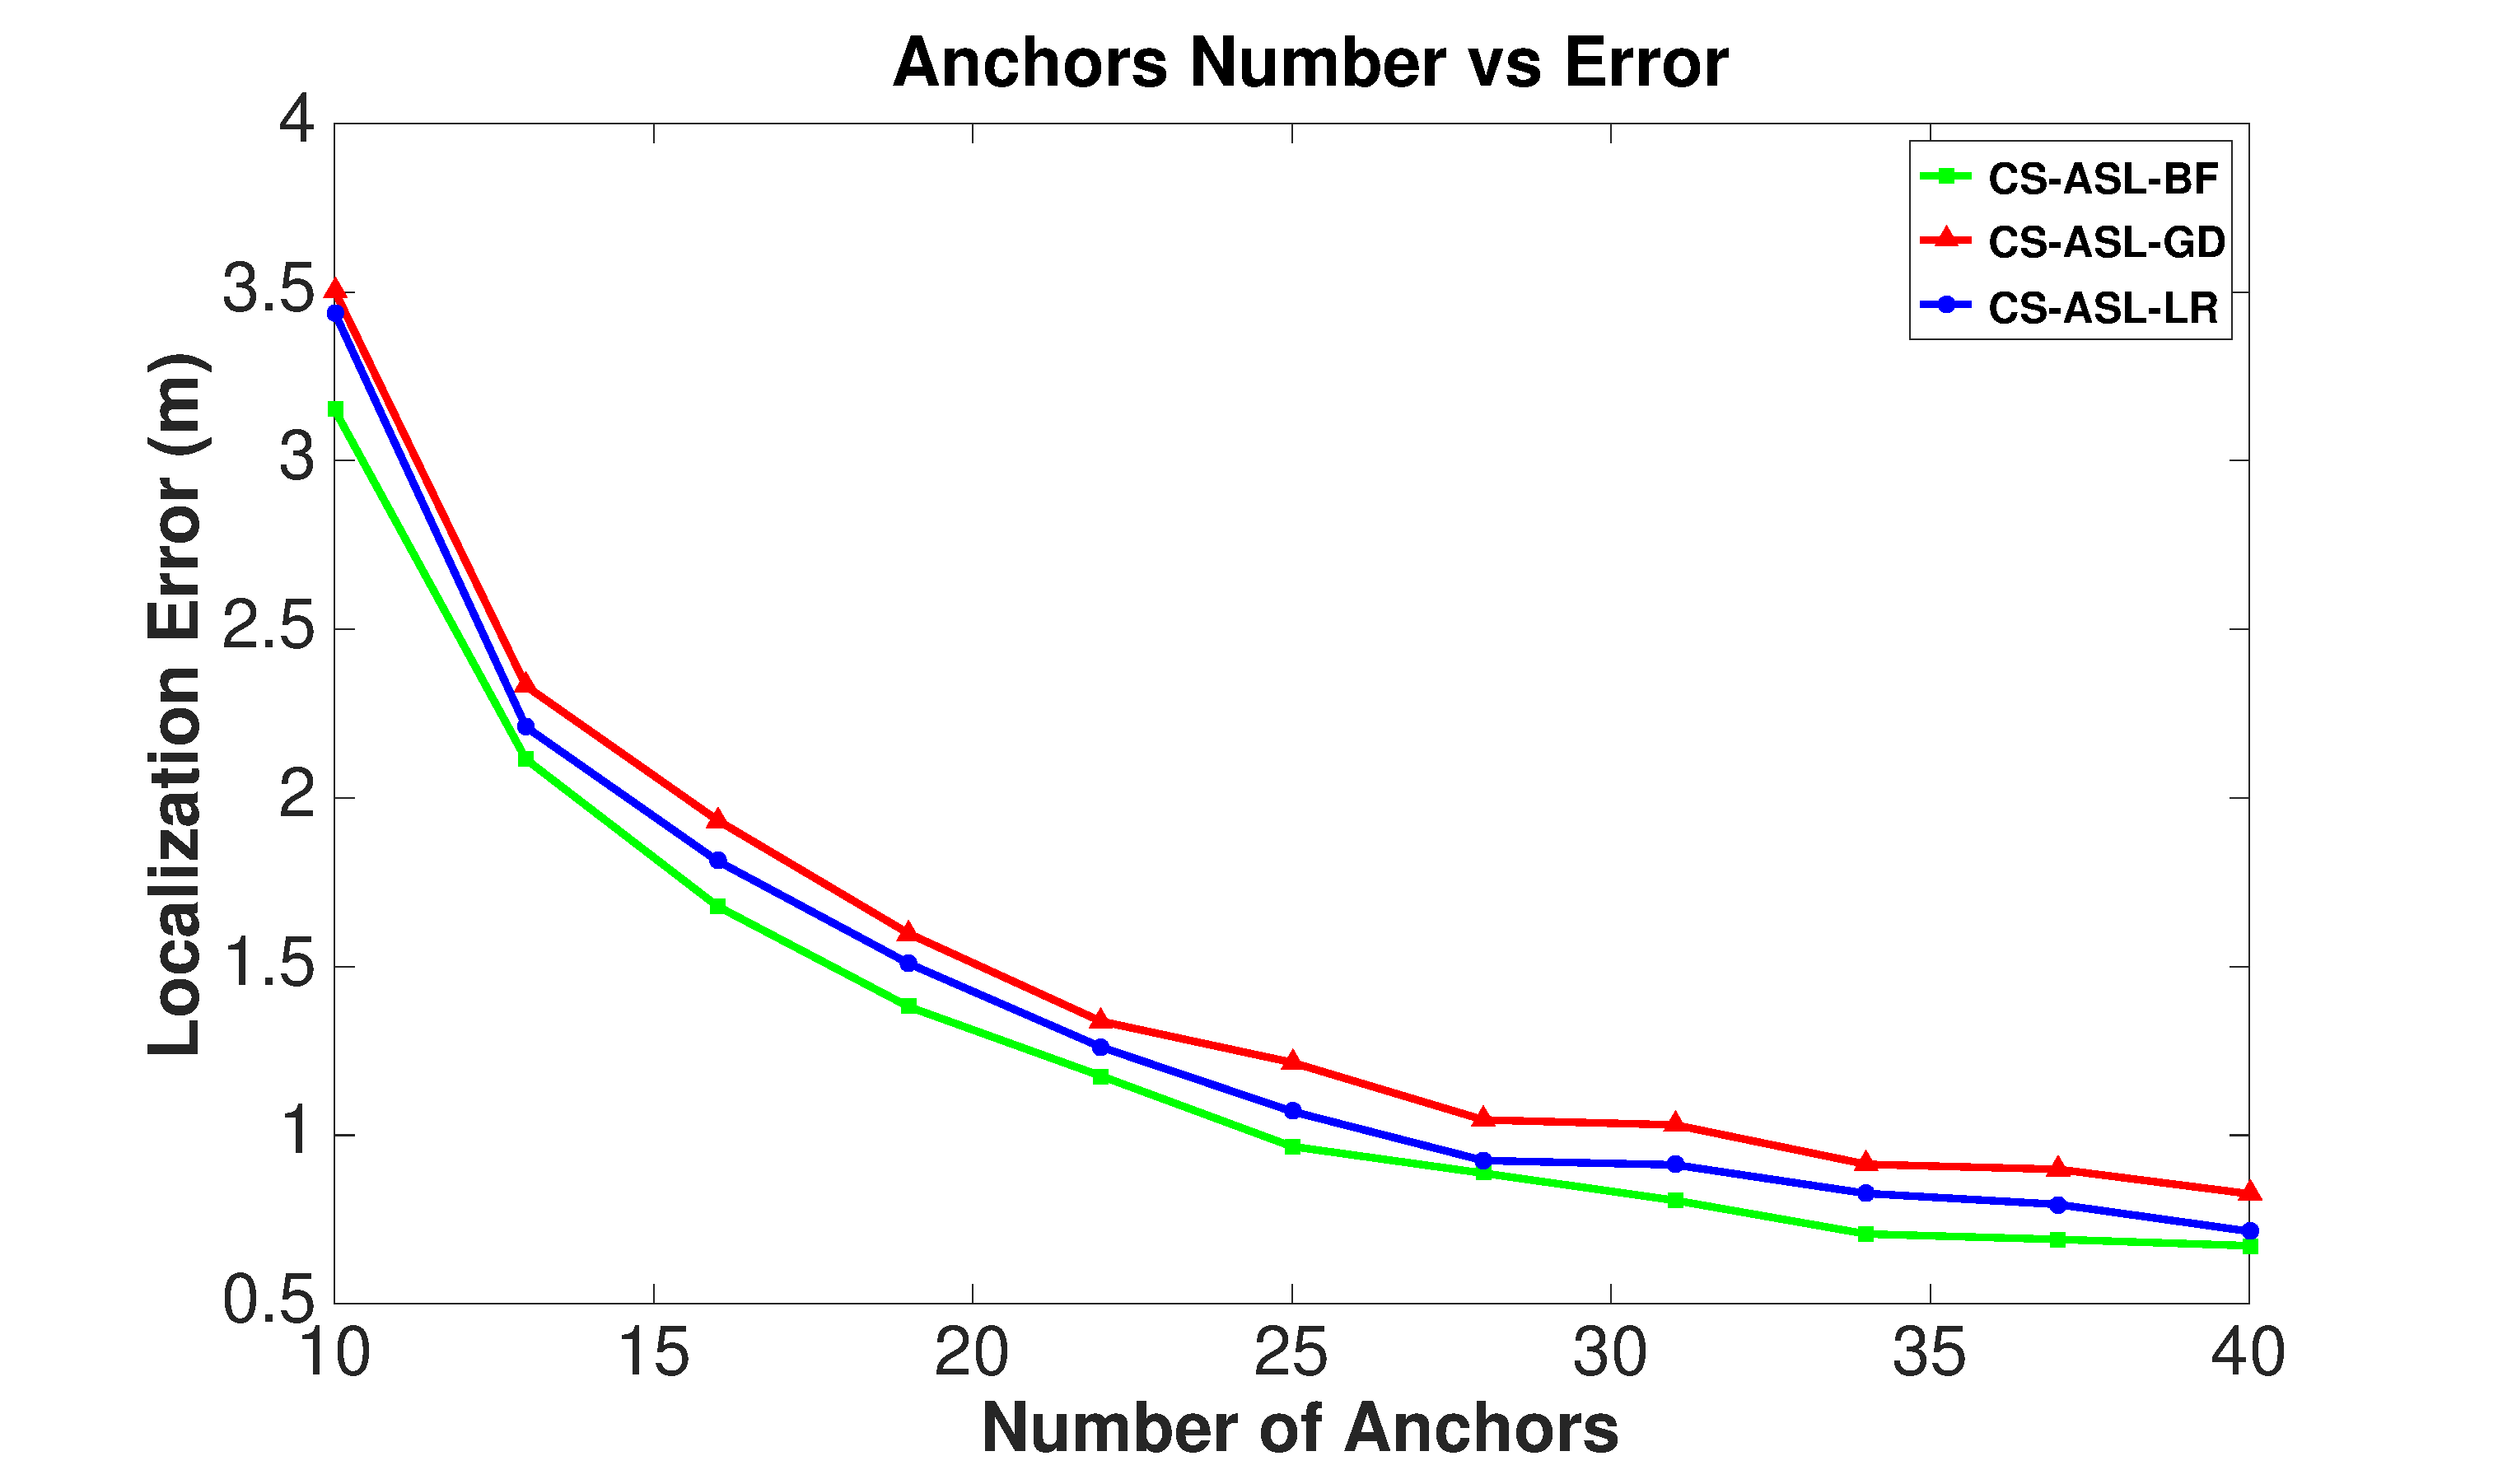
\includegraphics[height=5.0cm,width=7.0cm]{image/nodenumber.eps}
            \vspace{15mm}
            \caption{Localization Error vs. Number of Anchors}
             \vspace{-7mm}
             \label{fig4}
        \end{figure}
\fi
		
\textbf{2) Impact of the node location error:}
In this experiment we choose the location error from 0 to 0.5m in steps of 0.05m, other parameters remain the default. With the raisement of the node location error, Fig. \ref{Fig3:3-2} shows that the localization error increases slowly, even the error add to 0.5m our methods still have a good performance. 

\iffalse
  \begin{figure}[htb]
          %  \centering
		   \vspace{-25mm}
			 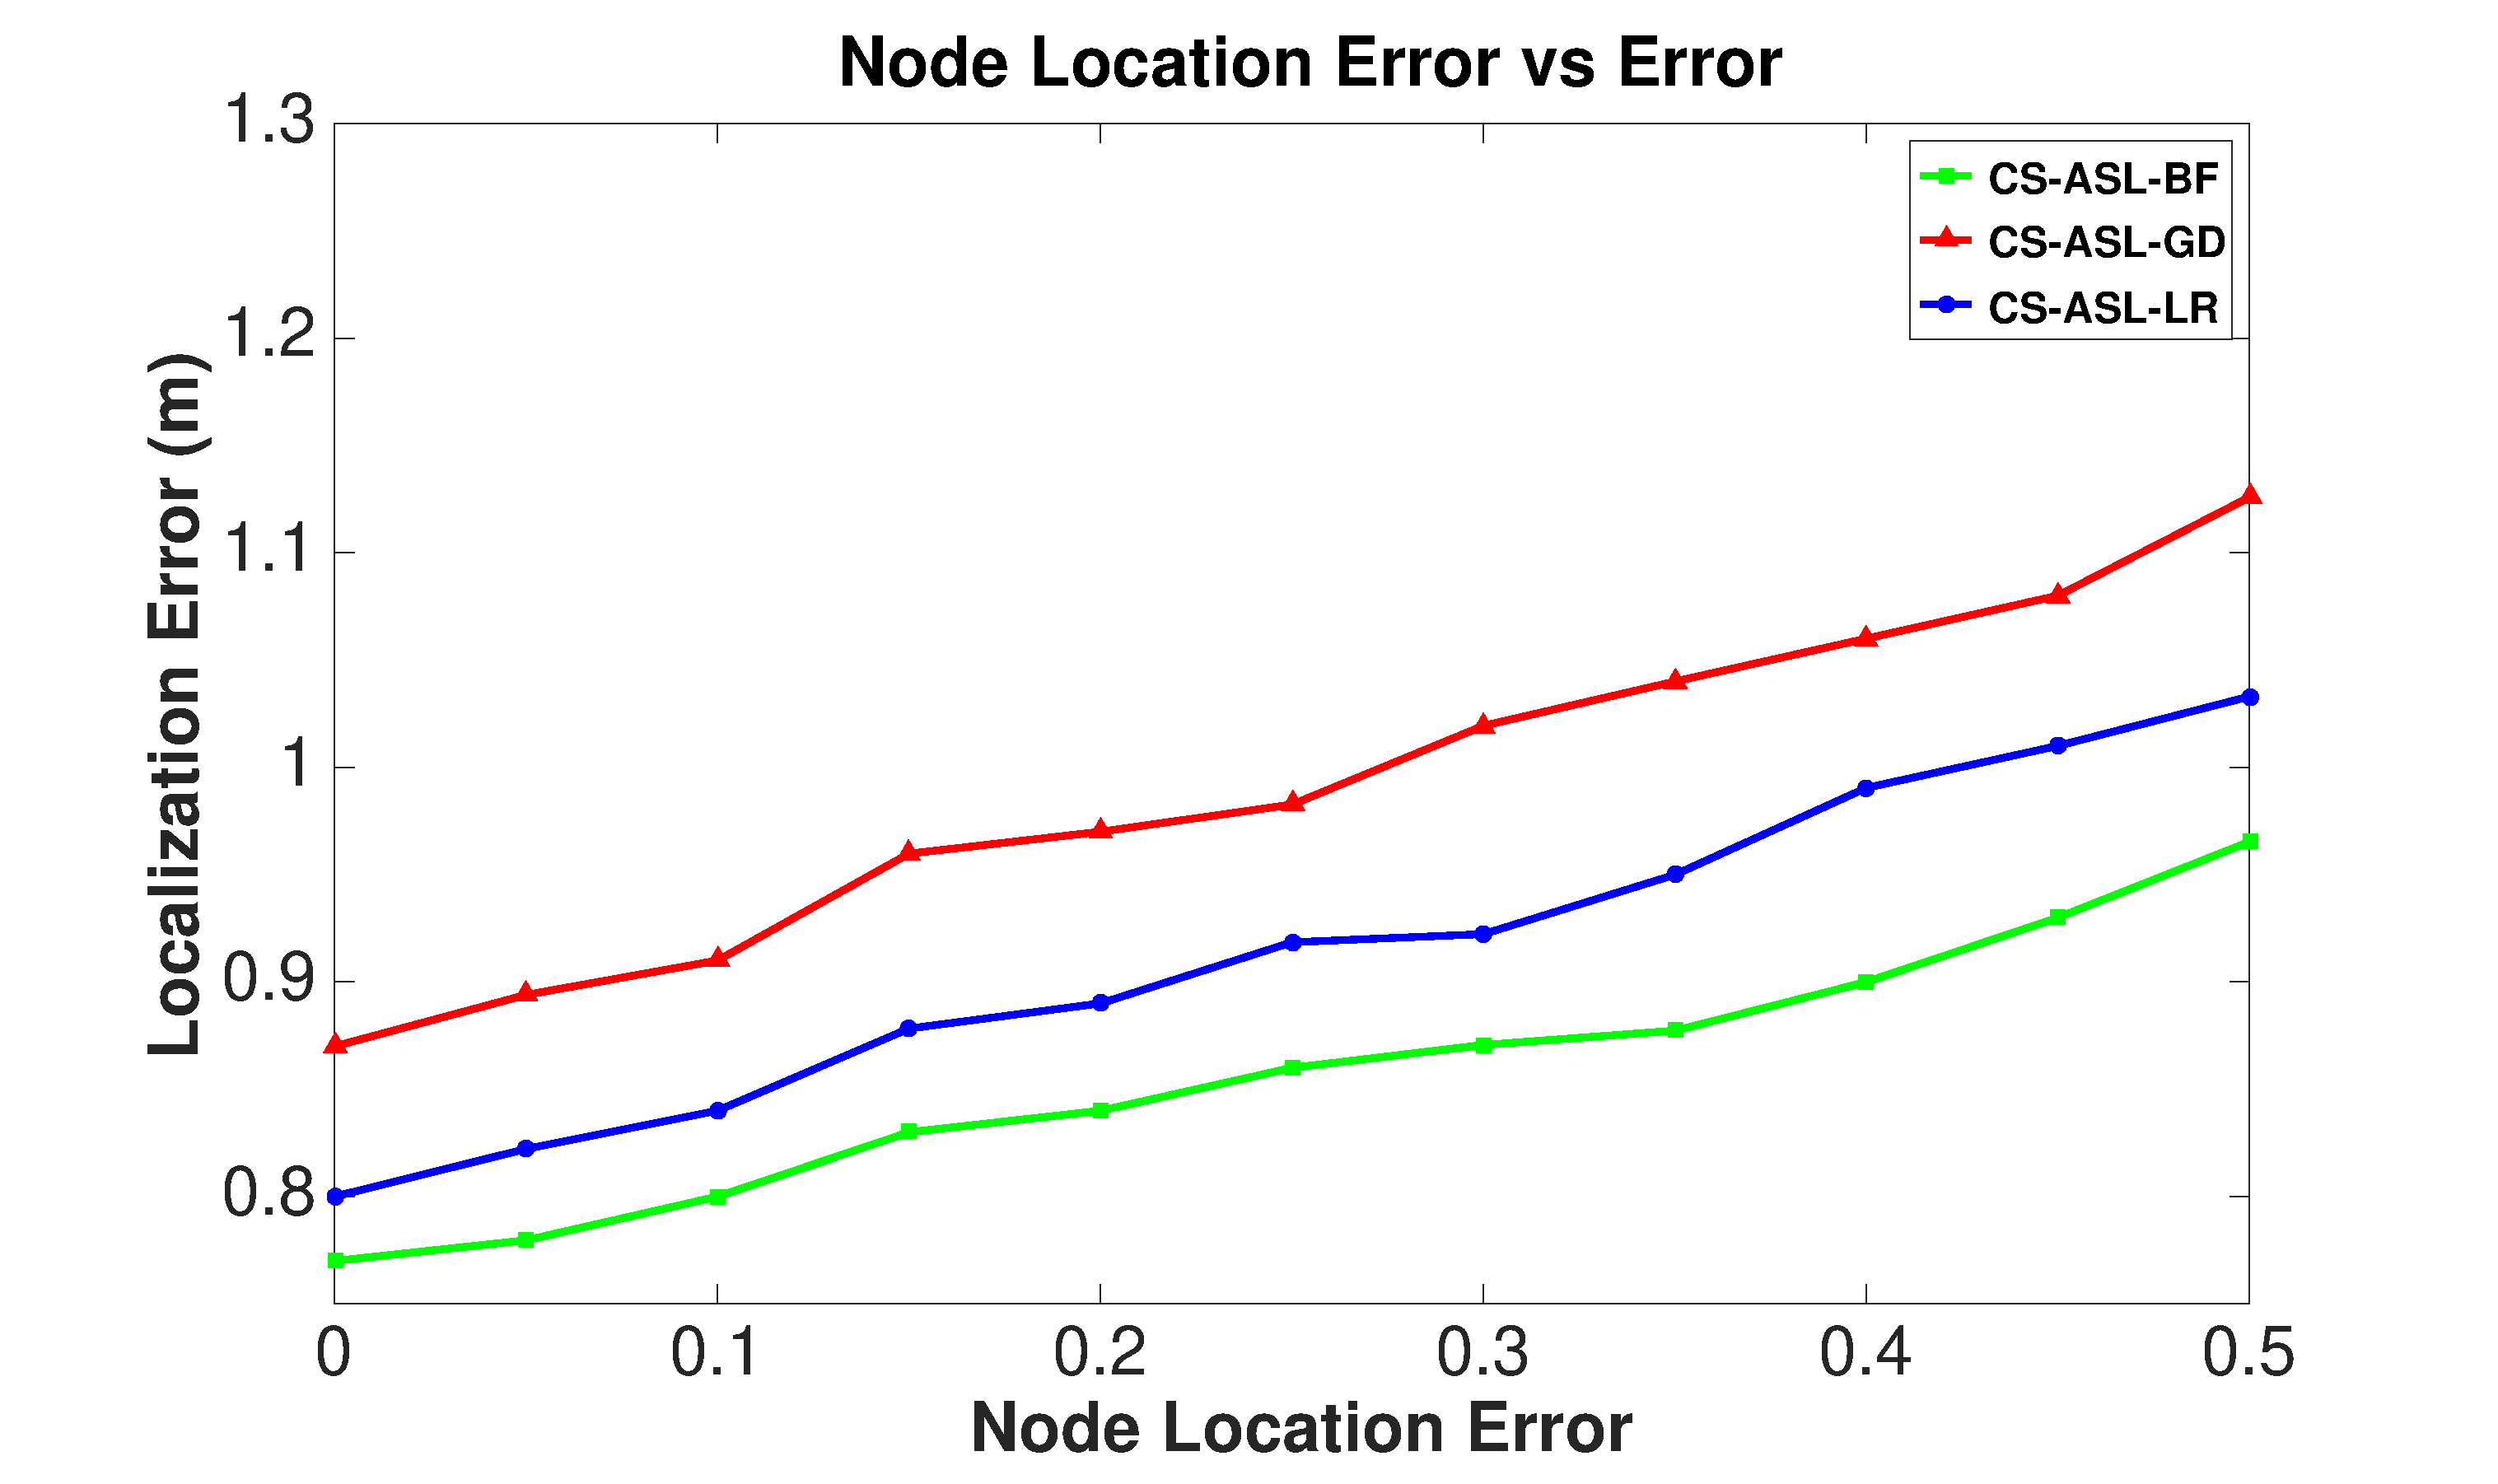
\includegraphics[height=5.0cm,width=7.0cm]{image/locationerror.eps}
            \vspace{25mm}
            \caption{Localization Error vs. Node Location Error}
             \vspace{-5mm}
             \label{fig5}
        \end{figure}
		\fi

\textbf{3) Impact of the node angle error:}
In localization system, node angel is also an essential parameter that influences the property. No matter how the sensor capability improves, the node angle error still exists due to magnetic interference or users' different operations. Here we choose the node angle error from 0 to 10$^{\circ} $ in steps of 1$^{\circ} $, other parameters still the default values.
As is shown in Fig. \ref{Fig3:3-3}, results demonstrate that our methods have a good node angle fault tolerance.

\textbf{4) Impact of bit-flipping number:}
In WASN, bit-flipping severely influences the localization performance. To prove our methods can  refine bit-fllipping, we reversal the 1-bit signals on purpose. In the condition of 30 nodes, we range the bit-flipping number from 0 to 10 in steps of 1, other parameter remain default. Result in Fig. \ref{Fig3:3-4} shows that CS-ASL-BF method performs well when bit-flipping occurs, on the basis of this,  CS-ASL-GD also have a certain ability to refine bit-flipping with the idea of final partly searching.
CS-ASL-LR behaves more approach to CS-ASL-BF method, even the bit-flipping number adds to 10, it can still determine the source location. Therefore, our methods are bit-flipping tolerance.

	\iffalse	
  \begin{figure}[htb]       
           % \centering
			\vspace{-15mm}
            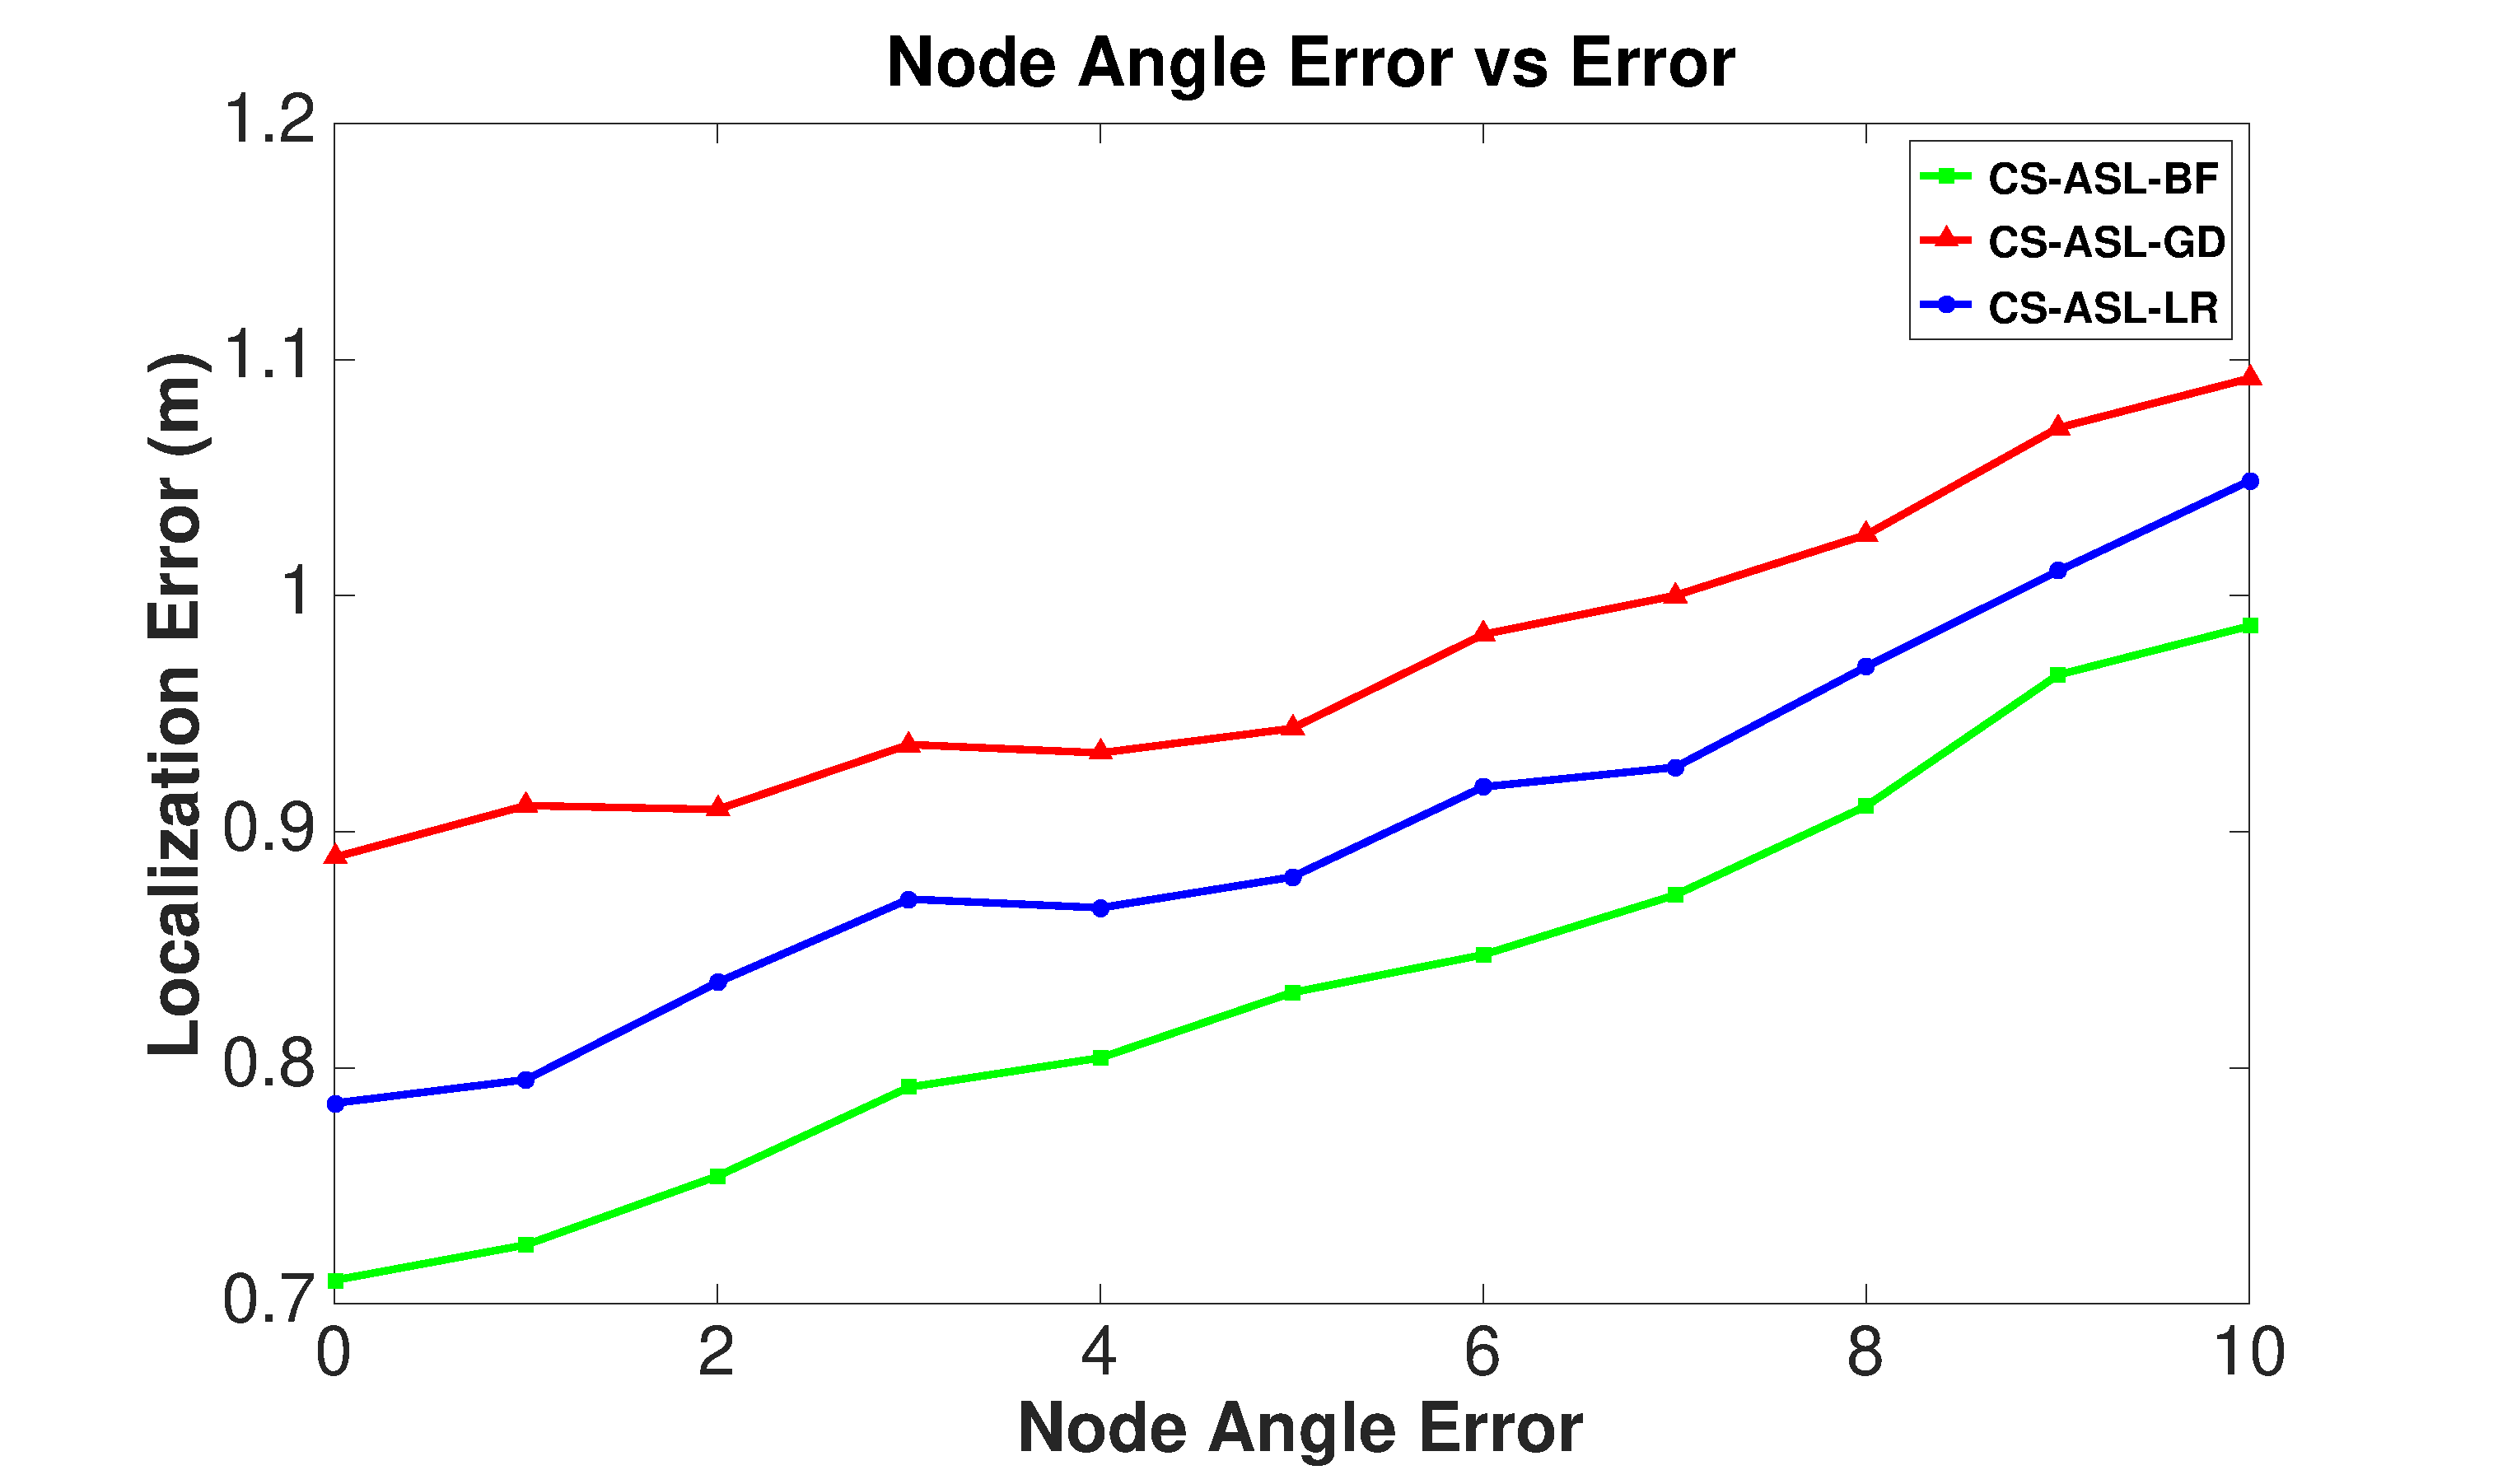
\includegraphics[height=5.0cm,width=7.0cm]{image/angle.eps}
           \vspace{15mm}
            \caption{Localization Error vs. Angle Error}
             \vspace{-5mm}
             \label{fig6}
        \end{figure}

\fi
		

%\subsection{Emulation}


%In this section, we reported system implementation of our design based on smartphone arrays.
%The 30 smartphones are deployed in a size of 16m$\times$10m space and connected by CISCO CVR328W-K9-CN wireless router.
%TPSN protocol is adapted in the proposed HPI-SBL system to realize time synchronization.
%In the experiment, smartphones are randomly deployed in the space, and 100 times localization results are shown in Fig.~\ref{Fig3:3-4}. 
%In the figure, blue squares stand for anchor
%nodes, red circle squares are the real position of acoustic sources and black dots are the estimated location by HPI-SBL. 
%An arrow origins from the estimated location of each acoustic source and points to its real position. 
%As shown in Fig.\ref{Fig3:3-4}, most of estimated locations are close to the ground truth and the errors between them are very small.
%In our experiment, the acoustic sources got localized with average and maximum error of 0.84 feet and 3.91 feet, respectively. Fig.\ref{Fig3:3-4} tells that
%the proposed HPI-SBL successfully accomplishes acoustic source localization with good robustness.

\iffalse
  \begin{figure}[htb]
              %    \centering
			    \vspace{-12mm}
            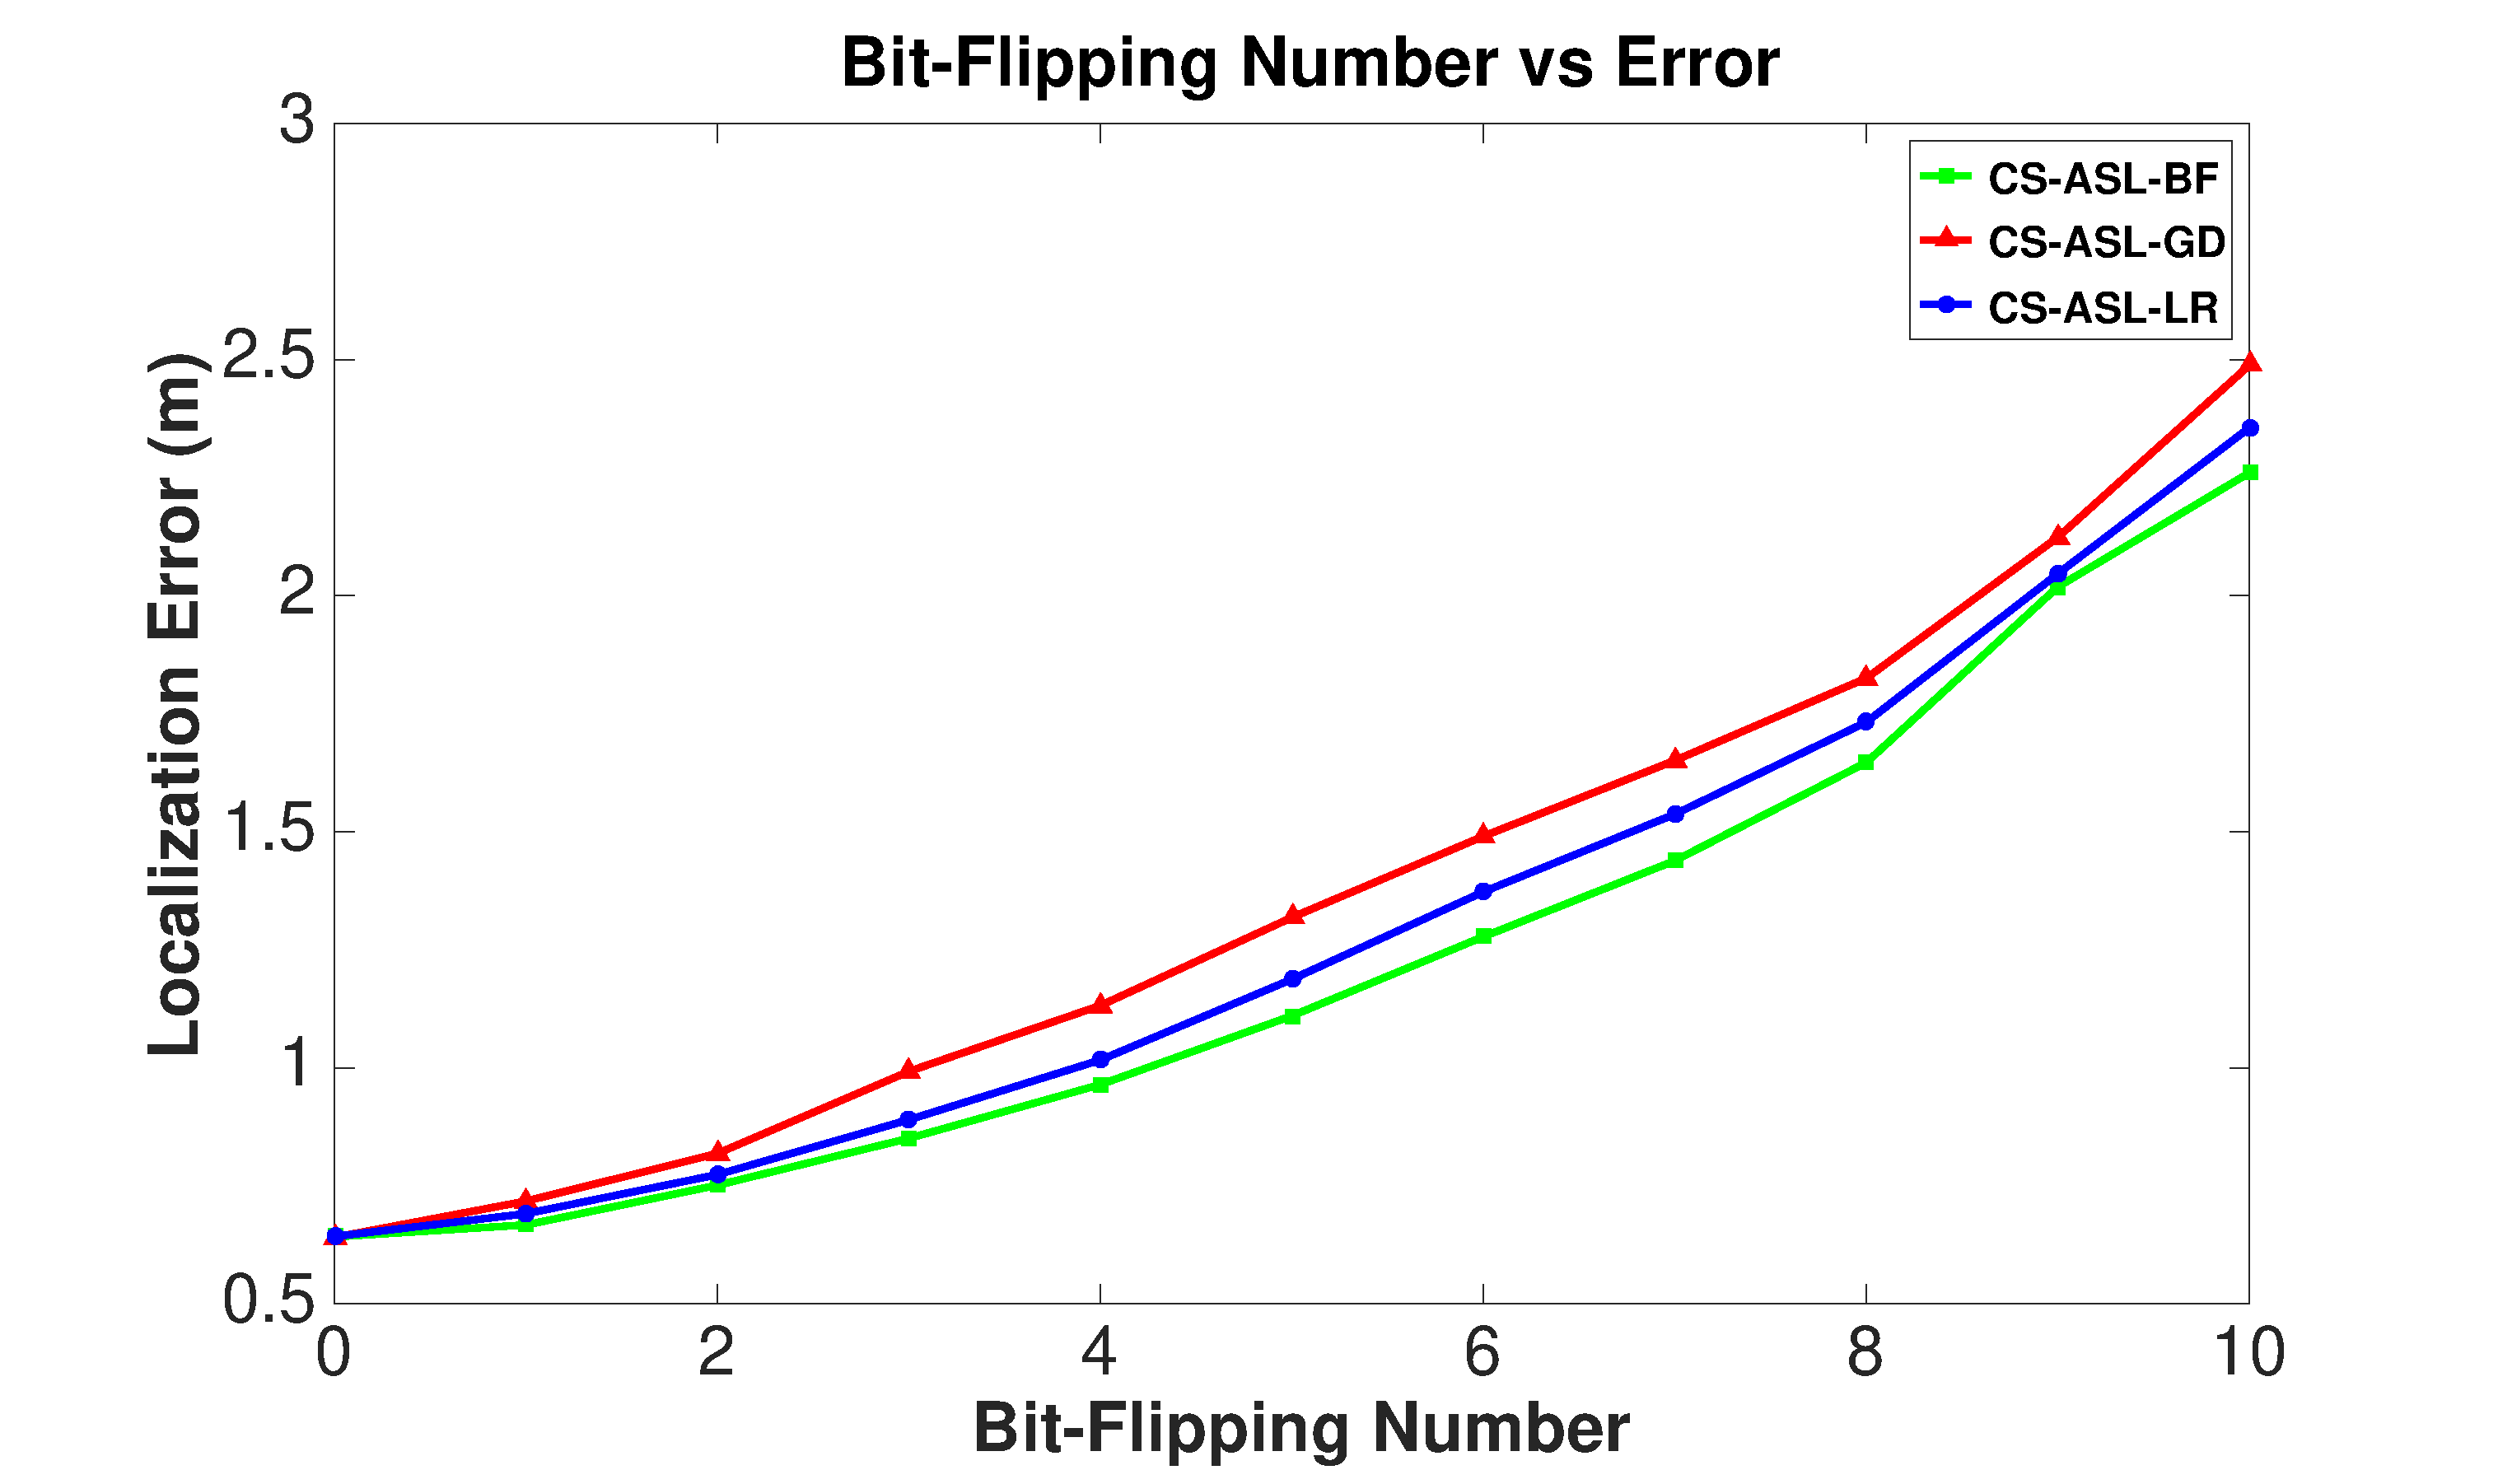
\includegraphics[height=5.0cm,width=7.0cm]{image/errornum.eps}
            \vspace{12mm}
            \caption{Localization Error vs. Error number}
             \vspace{-5mm}
             \label{fig7}
        \end{figure}
\fi
		
		
		
\begin{figure}[hptb]
\begin{center}
\subfigure[Impact of number of anchors]{
\label{Fig3:3-1}
\begin{minipage}[t]{0.46\linewidth}
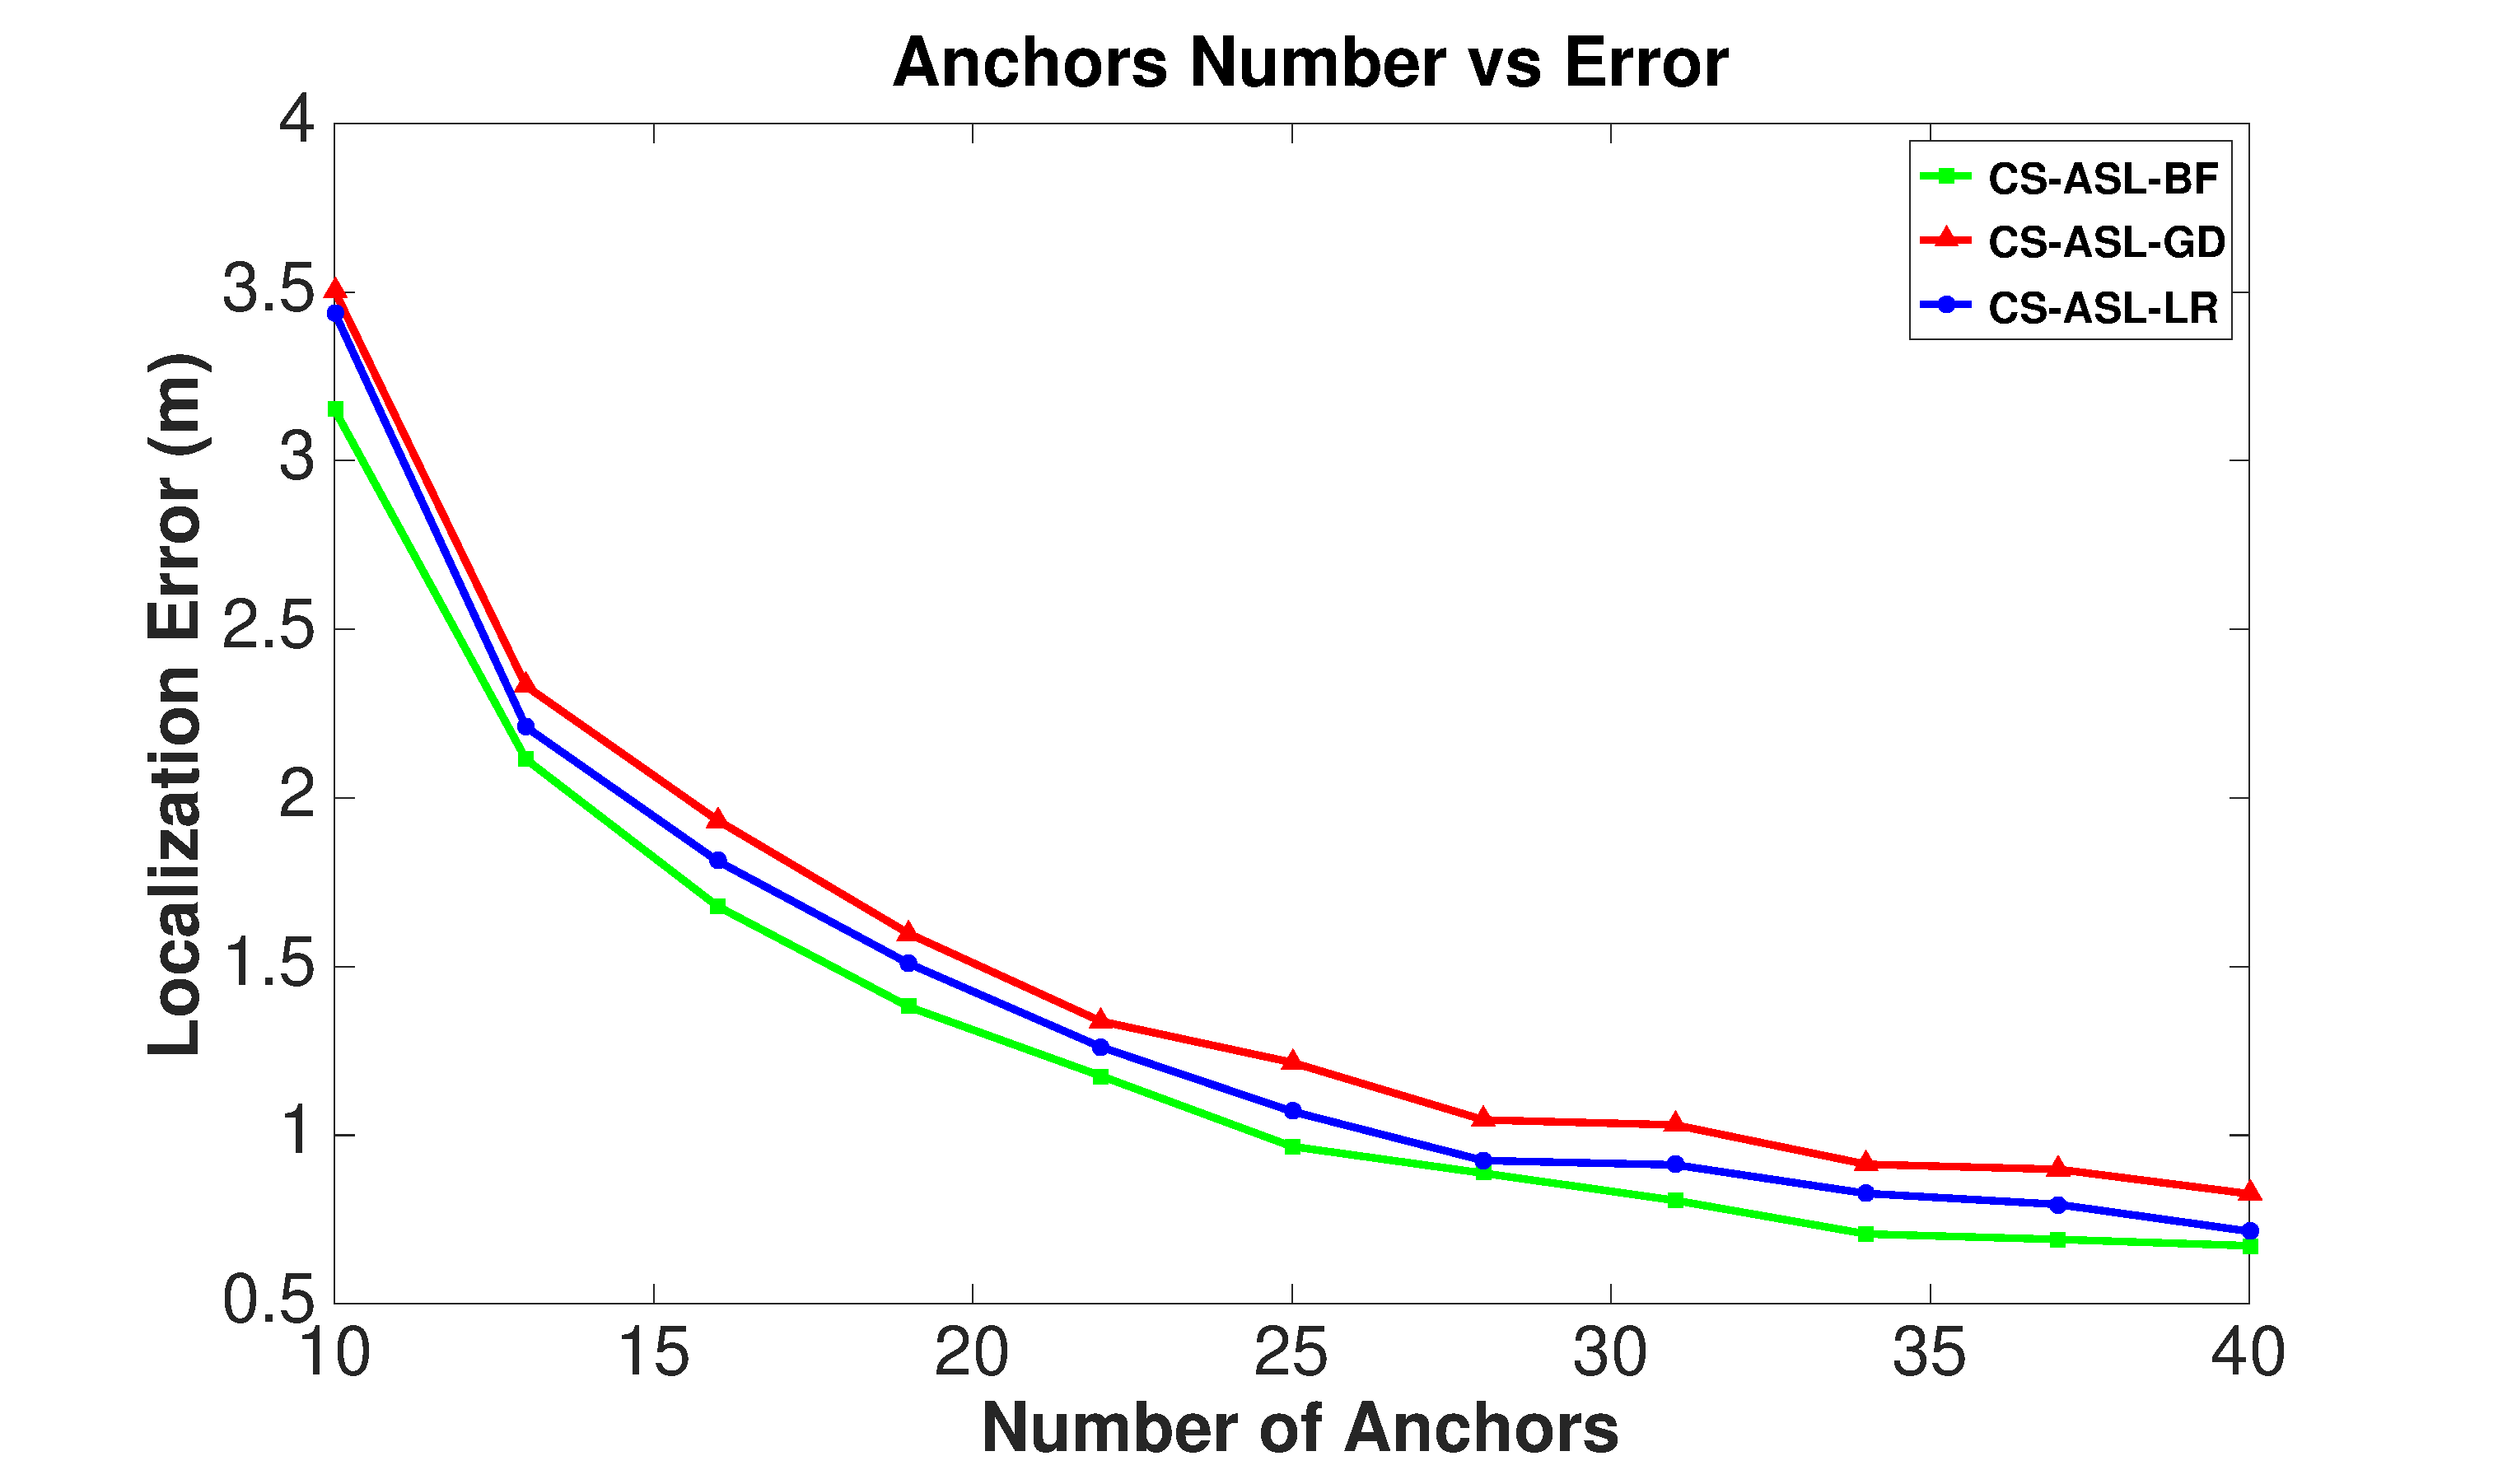
\includegraphics[width=1.150\textwidth]{image/nodenumber.eps}
\end{minipage}
}
\hspace{-0.1in}
\subfigure[Impact of node location error]{
\label{Fig3:3-2}
\begin{minipage}[t]{0.46\linewidth}
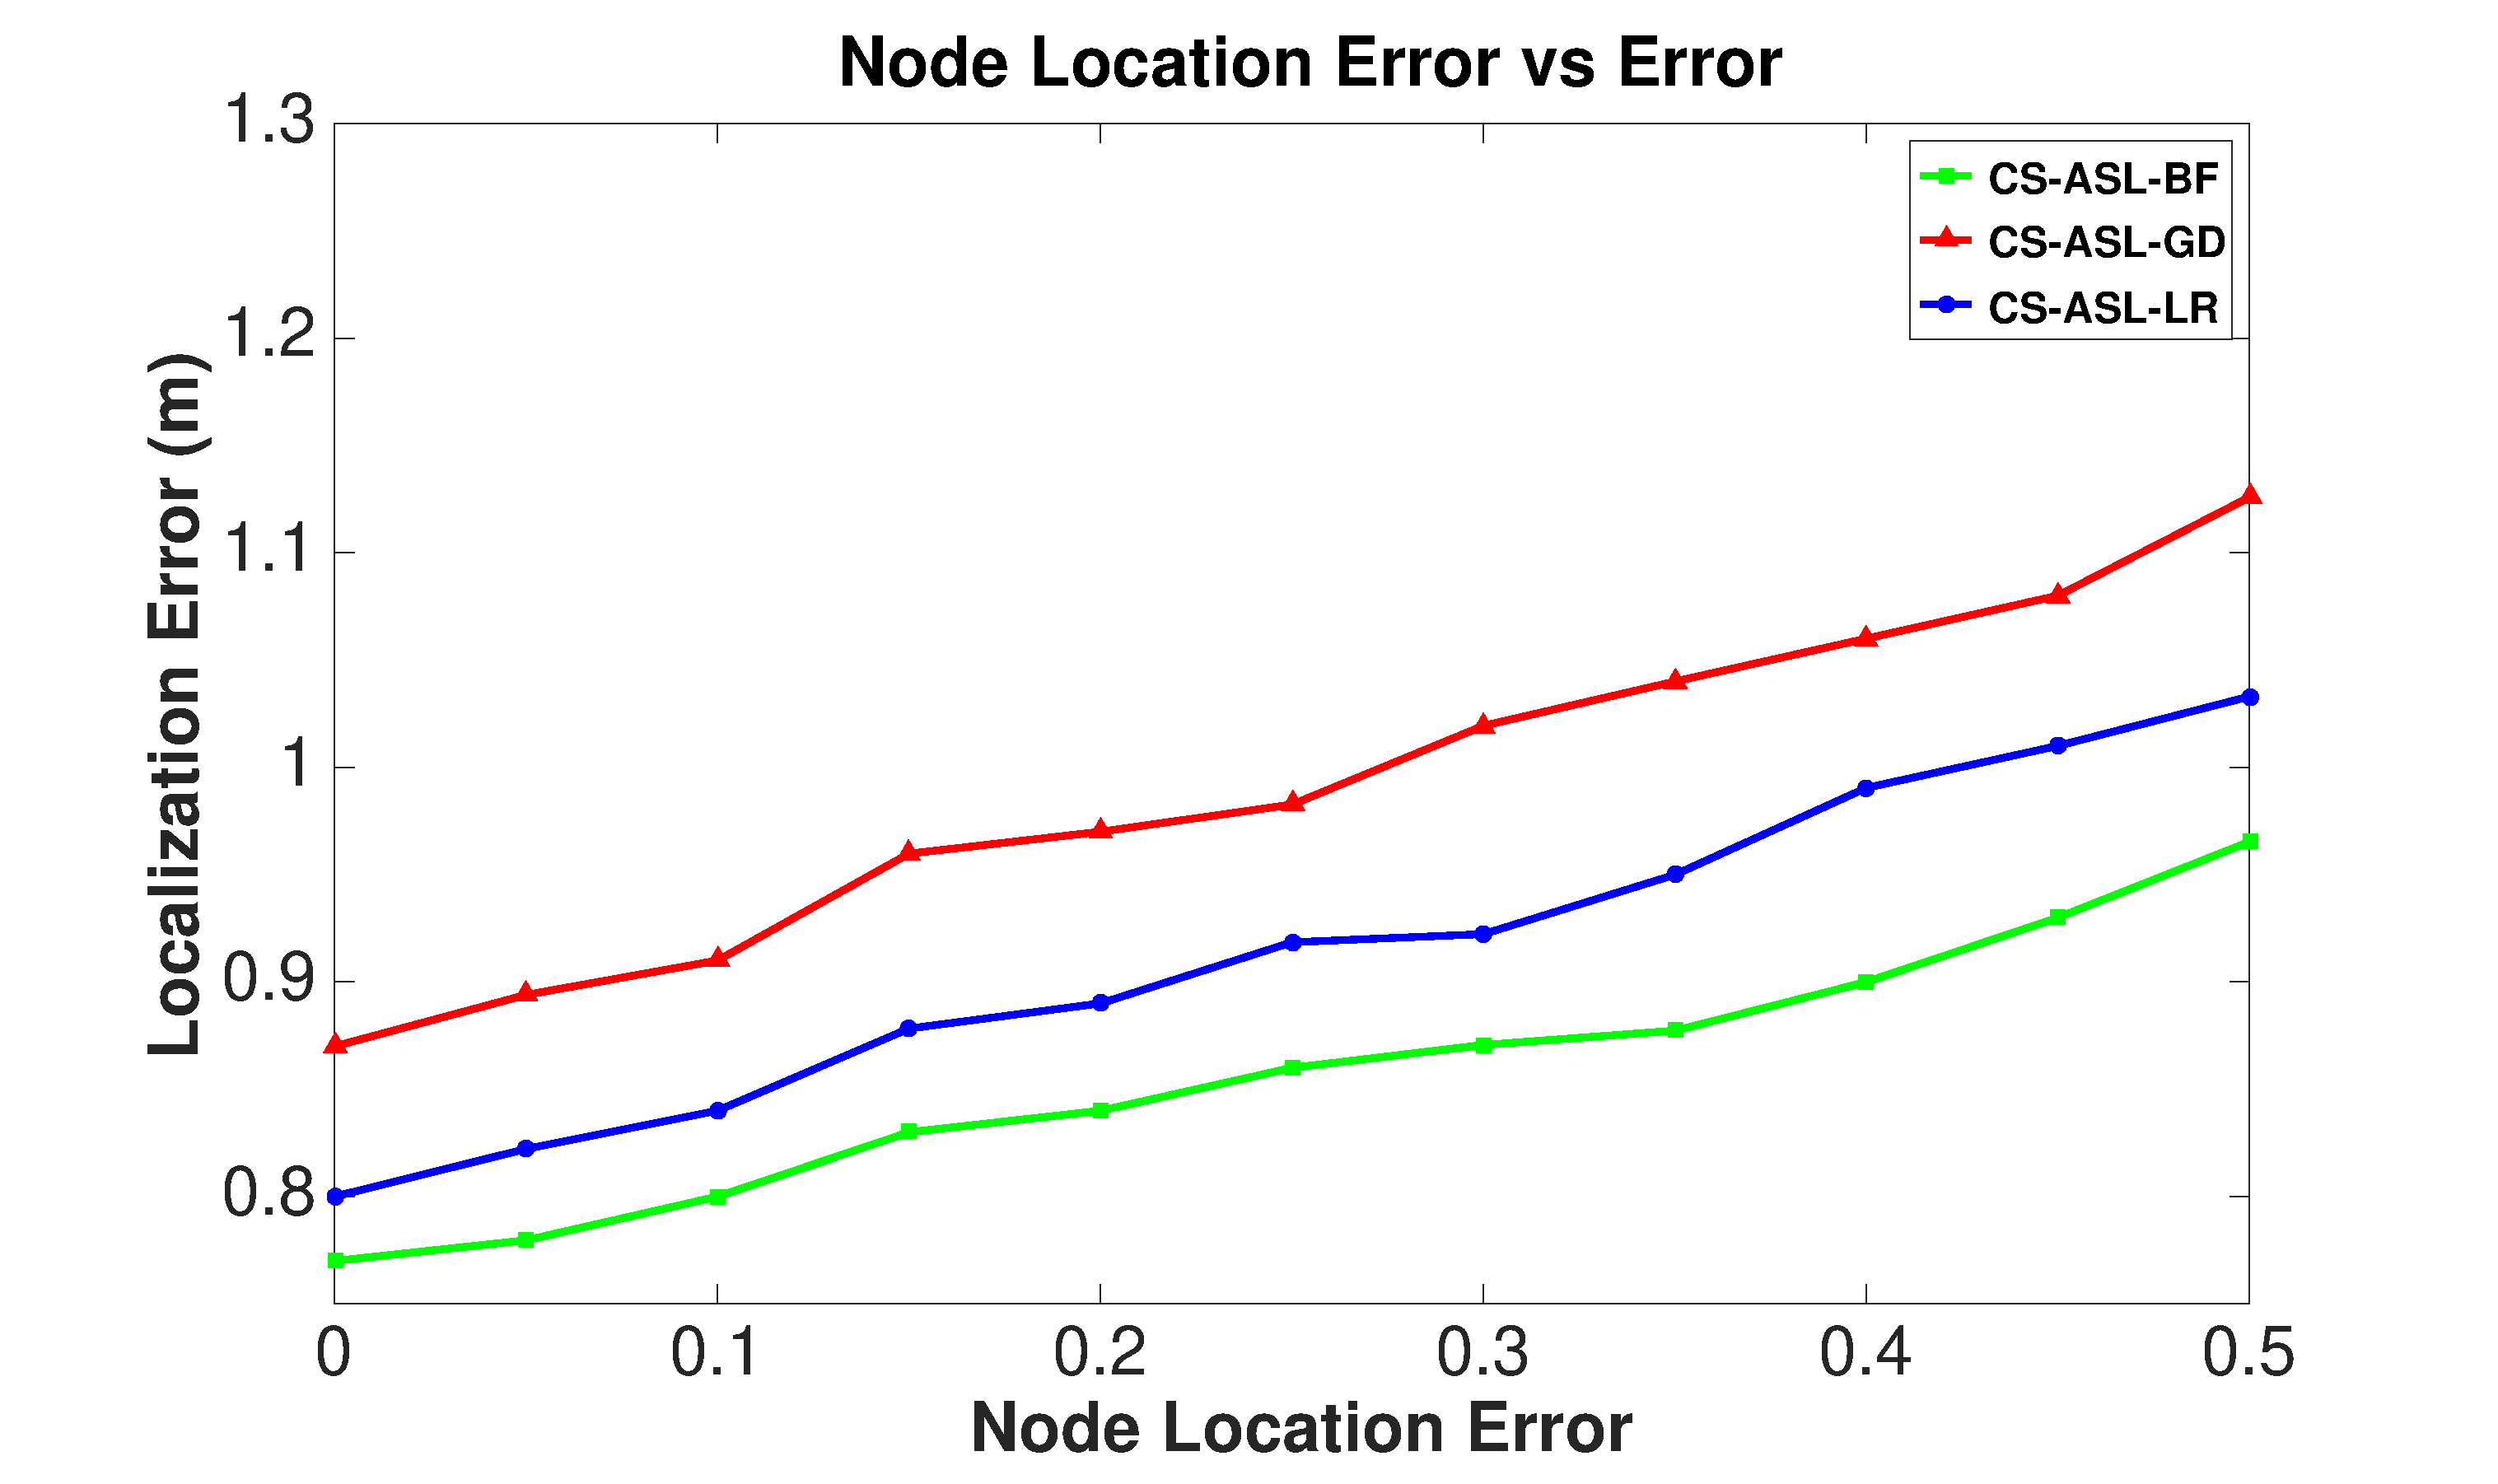
\includegraphics[width=1.150\textwidth]{image/locationerror.eps}
\end{minipage}
}

\subfigure[Impact of angle error]{
\label{Fig3:3-3}
\begin{minipage}[t]{0.46\linewidth}
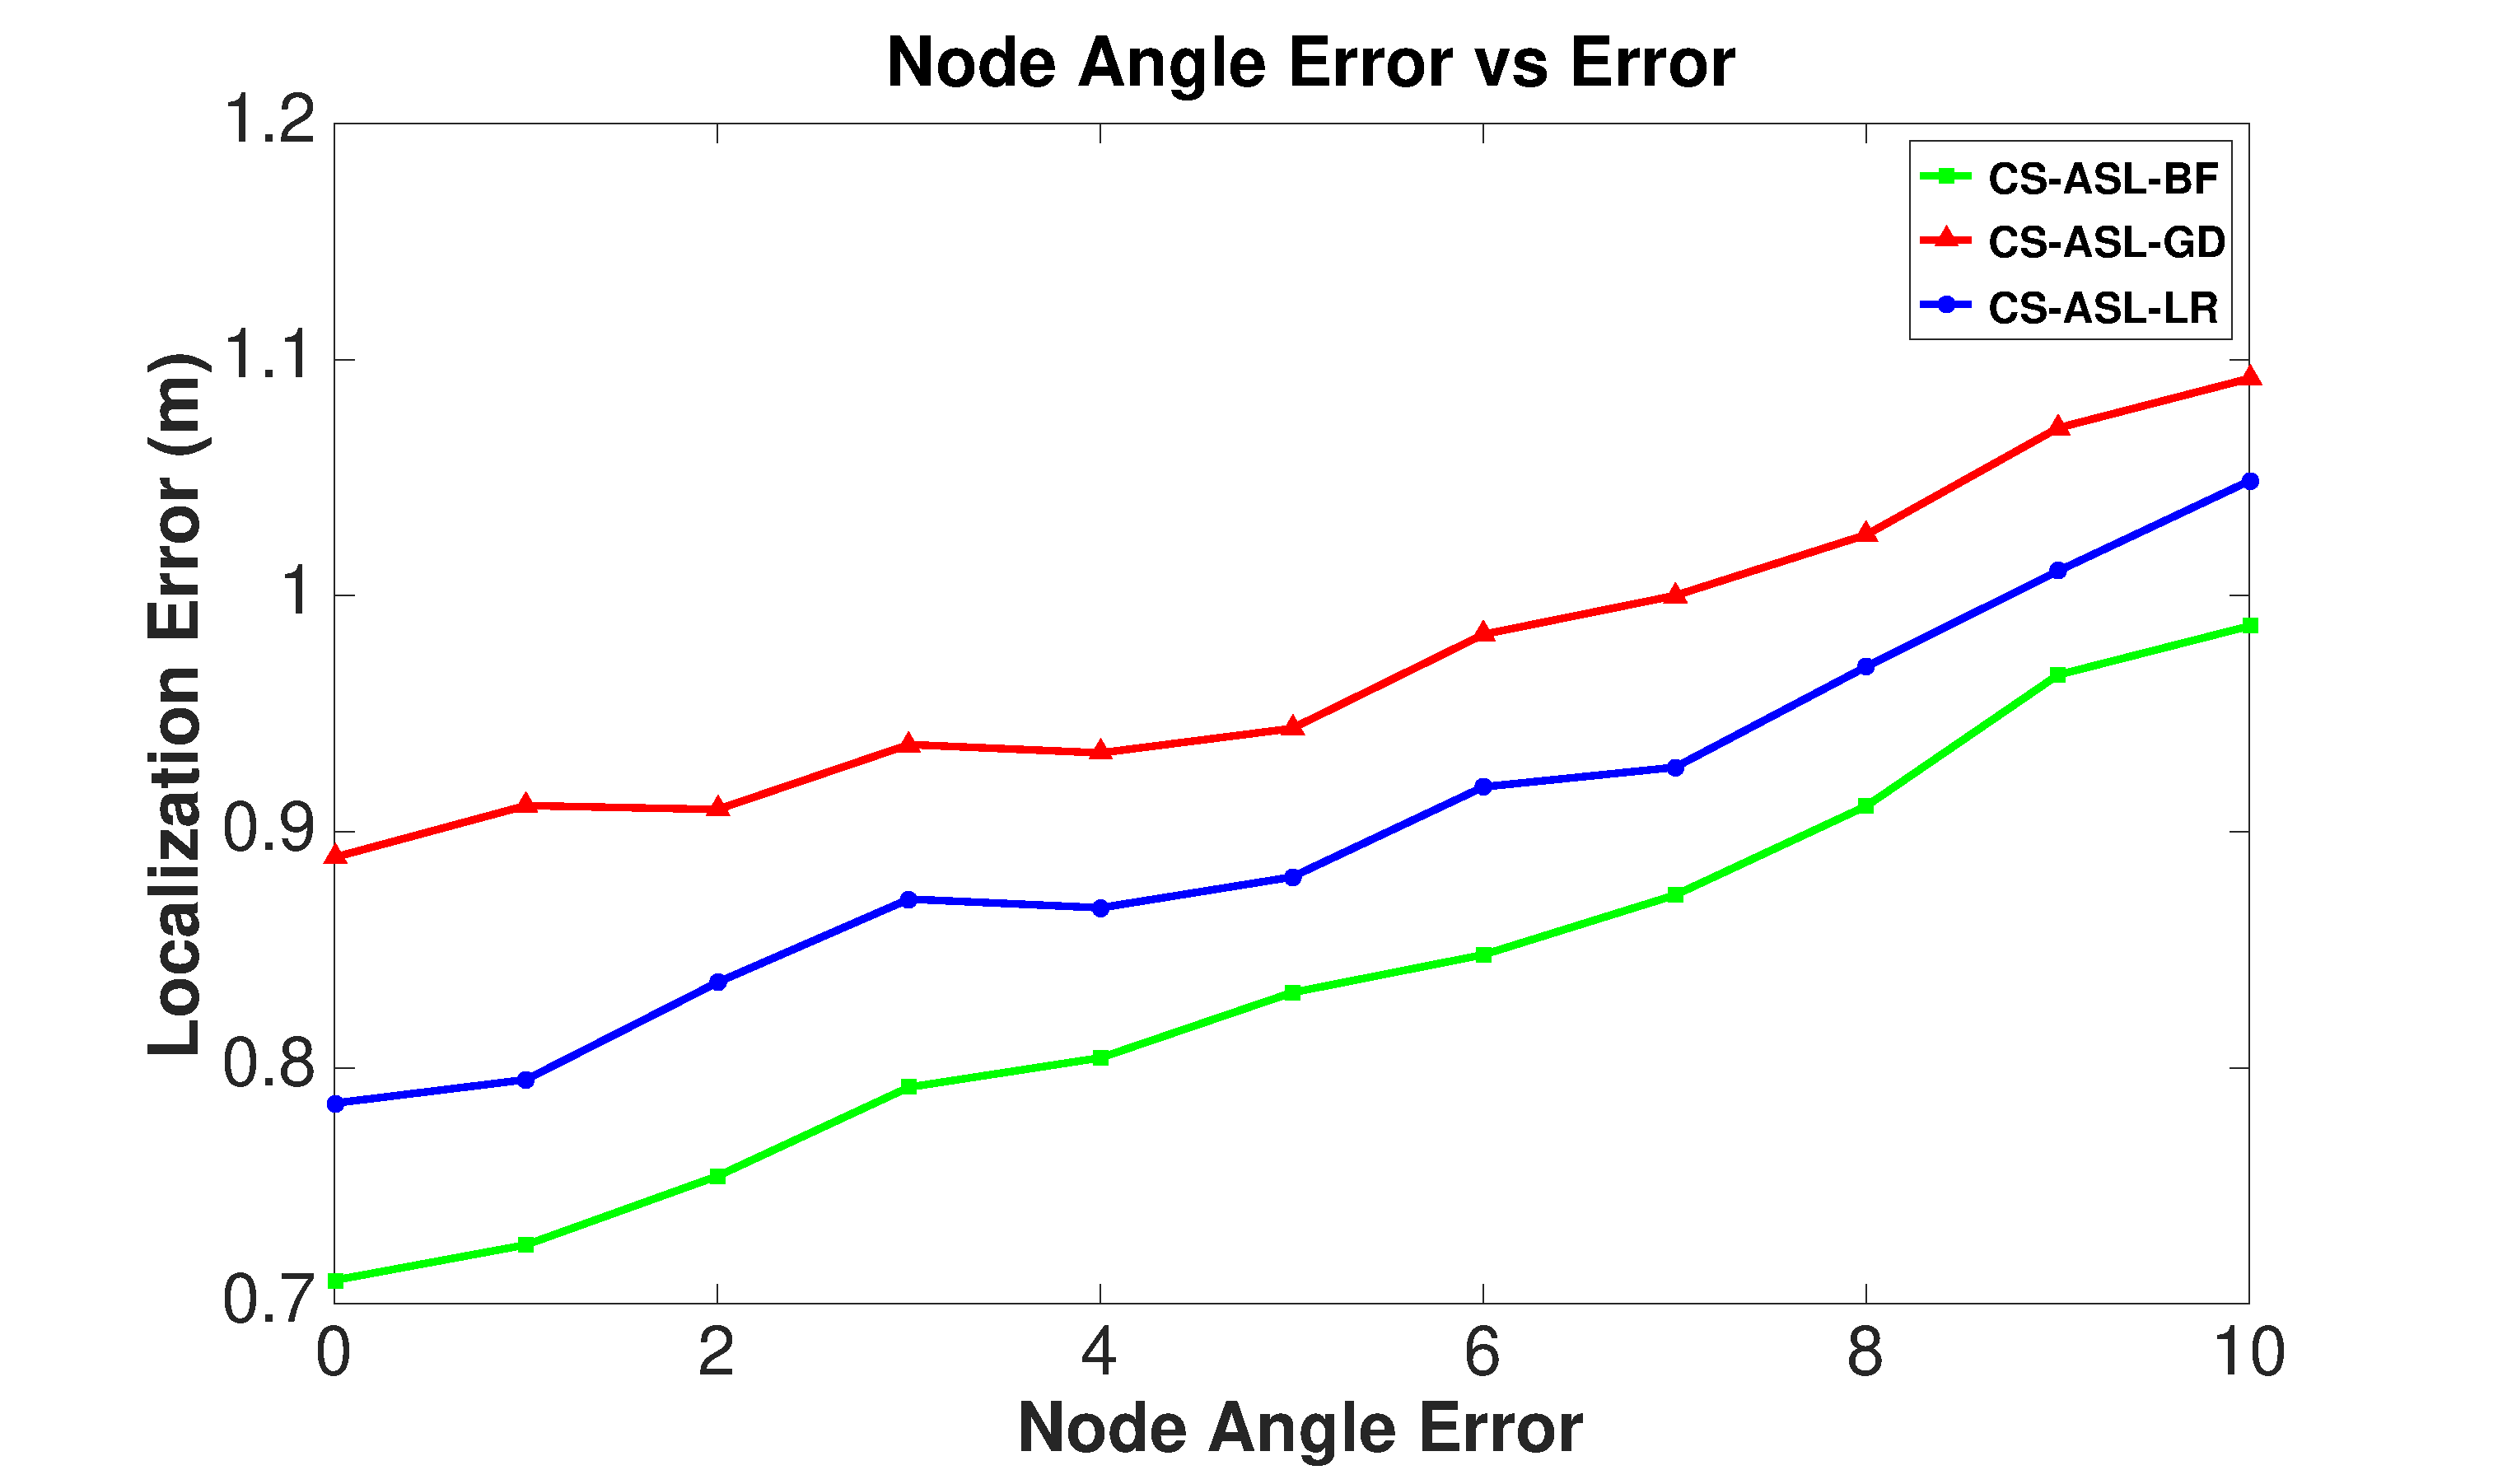
\includegraphics[width=1.150\textwidth]{image/angle.eps}
\end{minipage}
}
\hspace{-0.1in}
\subfigure[Impact of bit-flipping number]{
\label{Fig3:3-4}
\begin{minipage}[t]{0.46\linewidth}
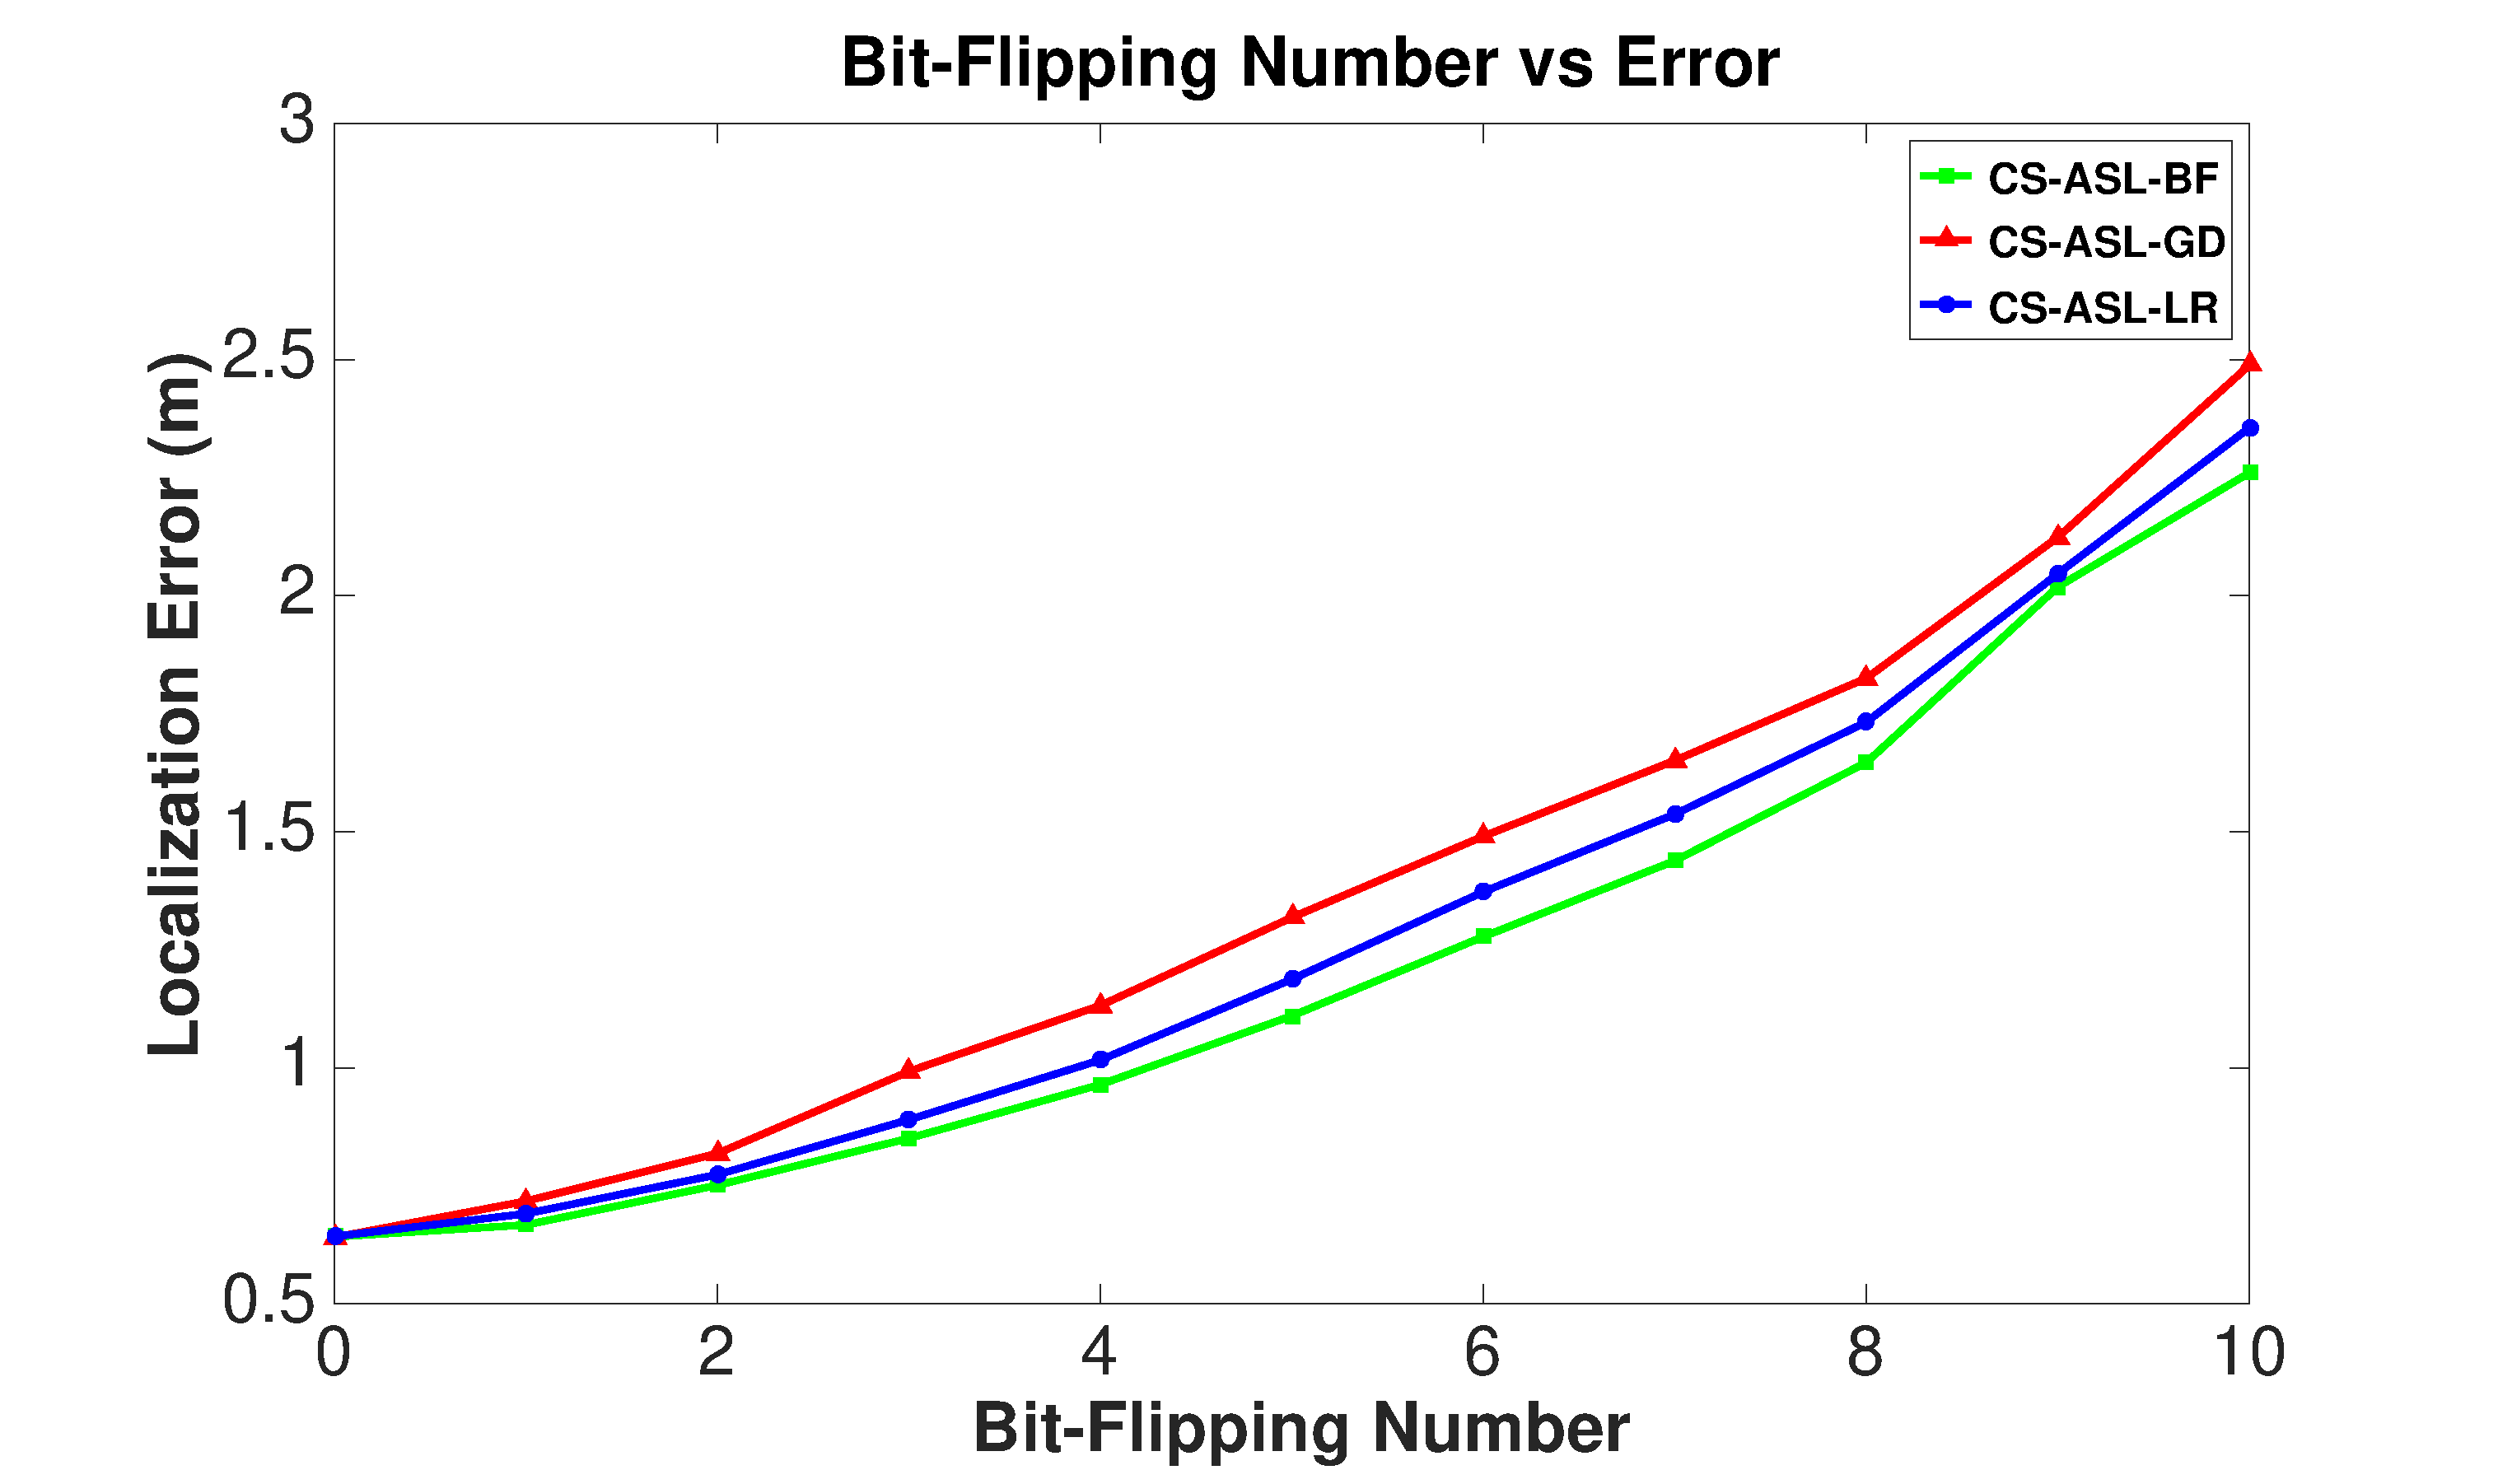
\includegraphics[width=1.150\textwidth]{image/errornum.eps}
\end{minipage}
}
\caption{\label{Fig3:}The results of simulation.}
\end{center}
 \vspace{-5mm}
\end{figure}

\subsection{Testbed Experiment}
In this part, we utilize the testbed experiment to evaluate the performance of our CS-ASL-LR method. We use 30 Redmi smartphones with double microphones as sensors to collect 1-bit datas and connect them through TP-LINK TL-WDR4310 wireless router. We do the experiments for 100 times, every time we deployed the 30 smartphones randomly in an area of 16m$\times$10m, results are demonstrated in Fig.3, blue squares stand for anchor nodes, red circle squares denote the real acoustic sources position and black dots are the estimated location by CS-ASL-LR. An arrow origins from the estimated location of each acoustic source and points to its real position. As shown in Fig.3, most of the estimated locations are close to the ground truth and the errors between them are very small. In our experiment, the acoustic sources got localized with average and maximum error of 0.63 feet and 2.74 feet, respectively. Fig.3 tells that the proposed CS-ASL-LR successfully accomplishes acoustic source localization.

\begin{figure}[htb]
	\centering
	%\setlength{\abovecaptionskip}{-15pt}
	%\setlength{\belowcaptionskip}{-5pt}
	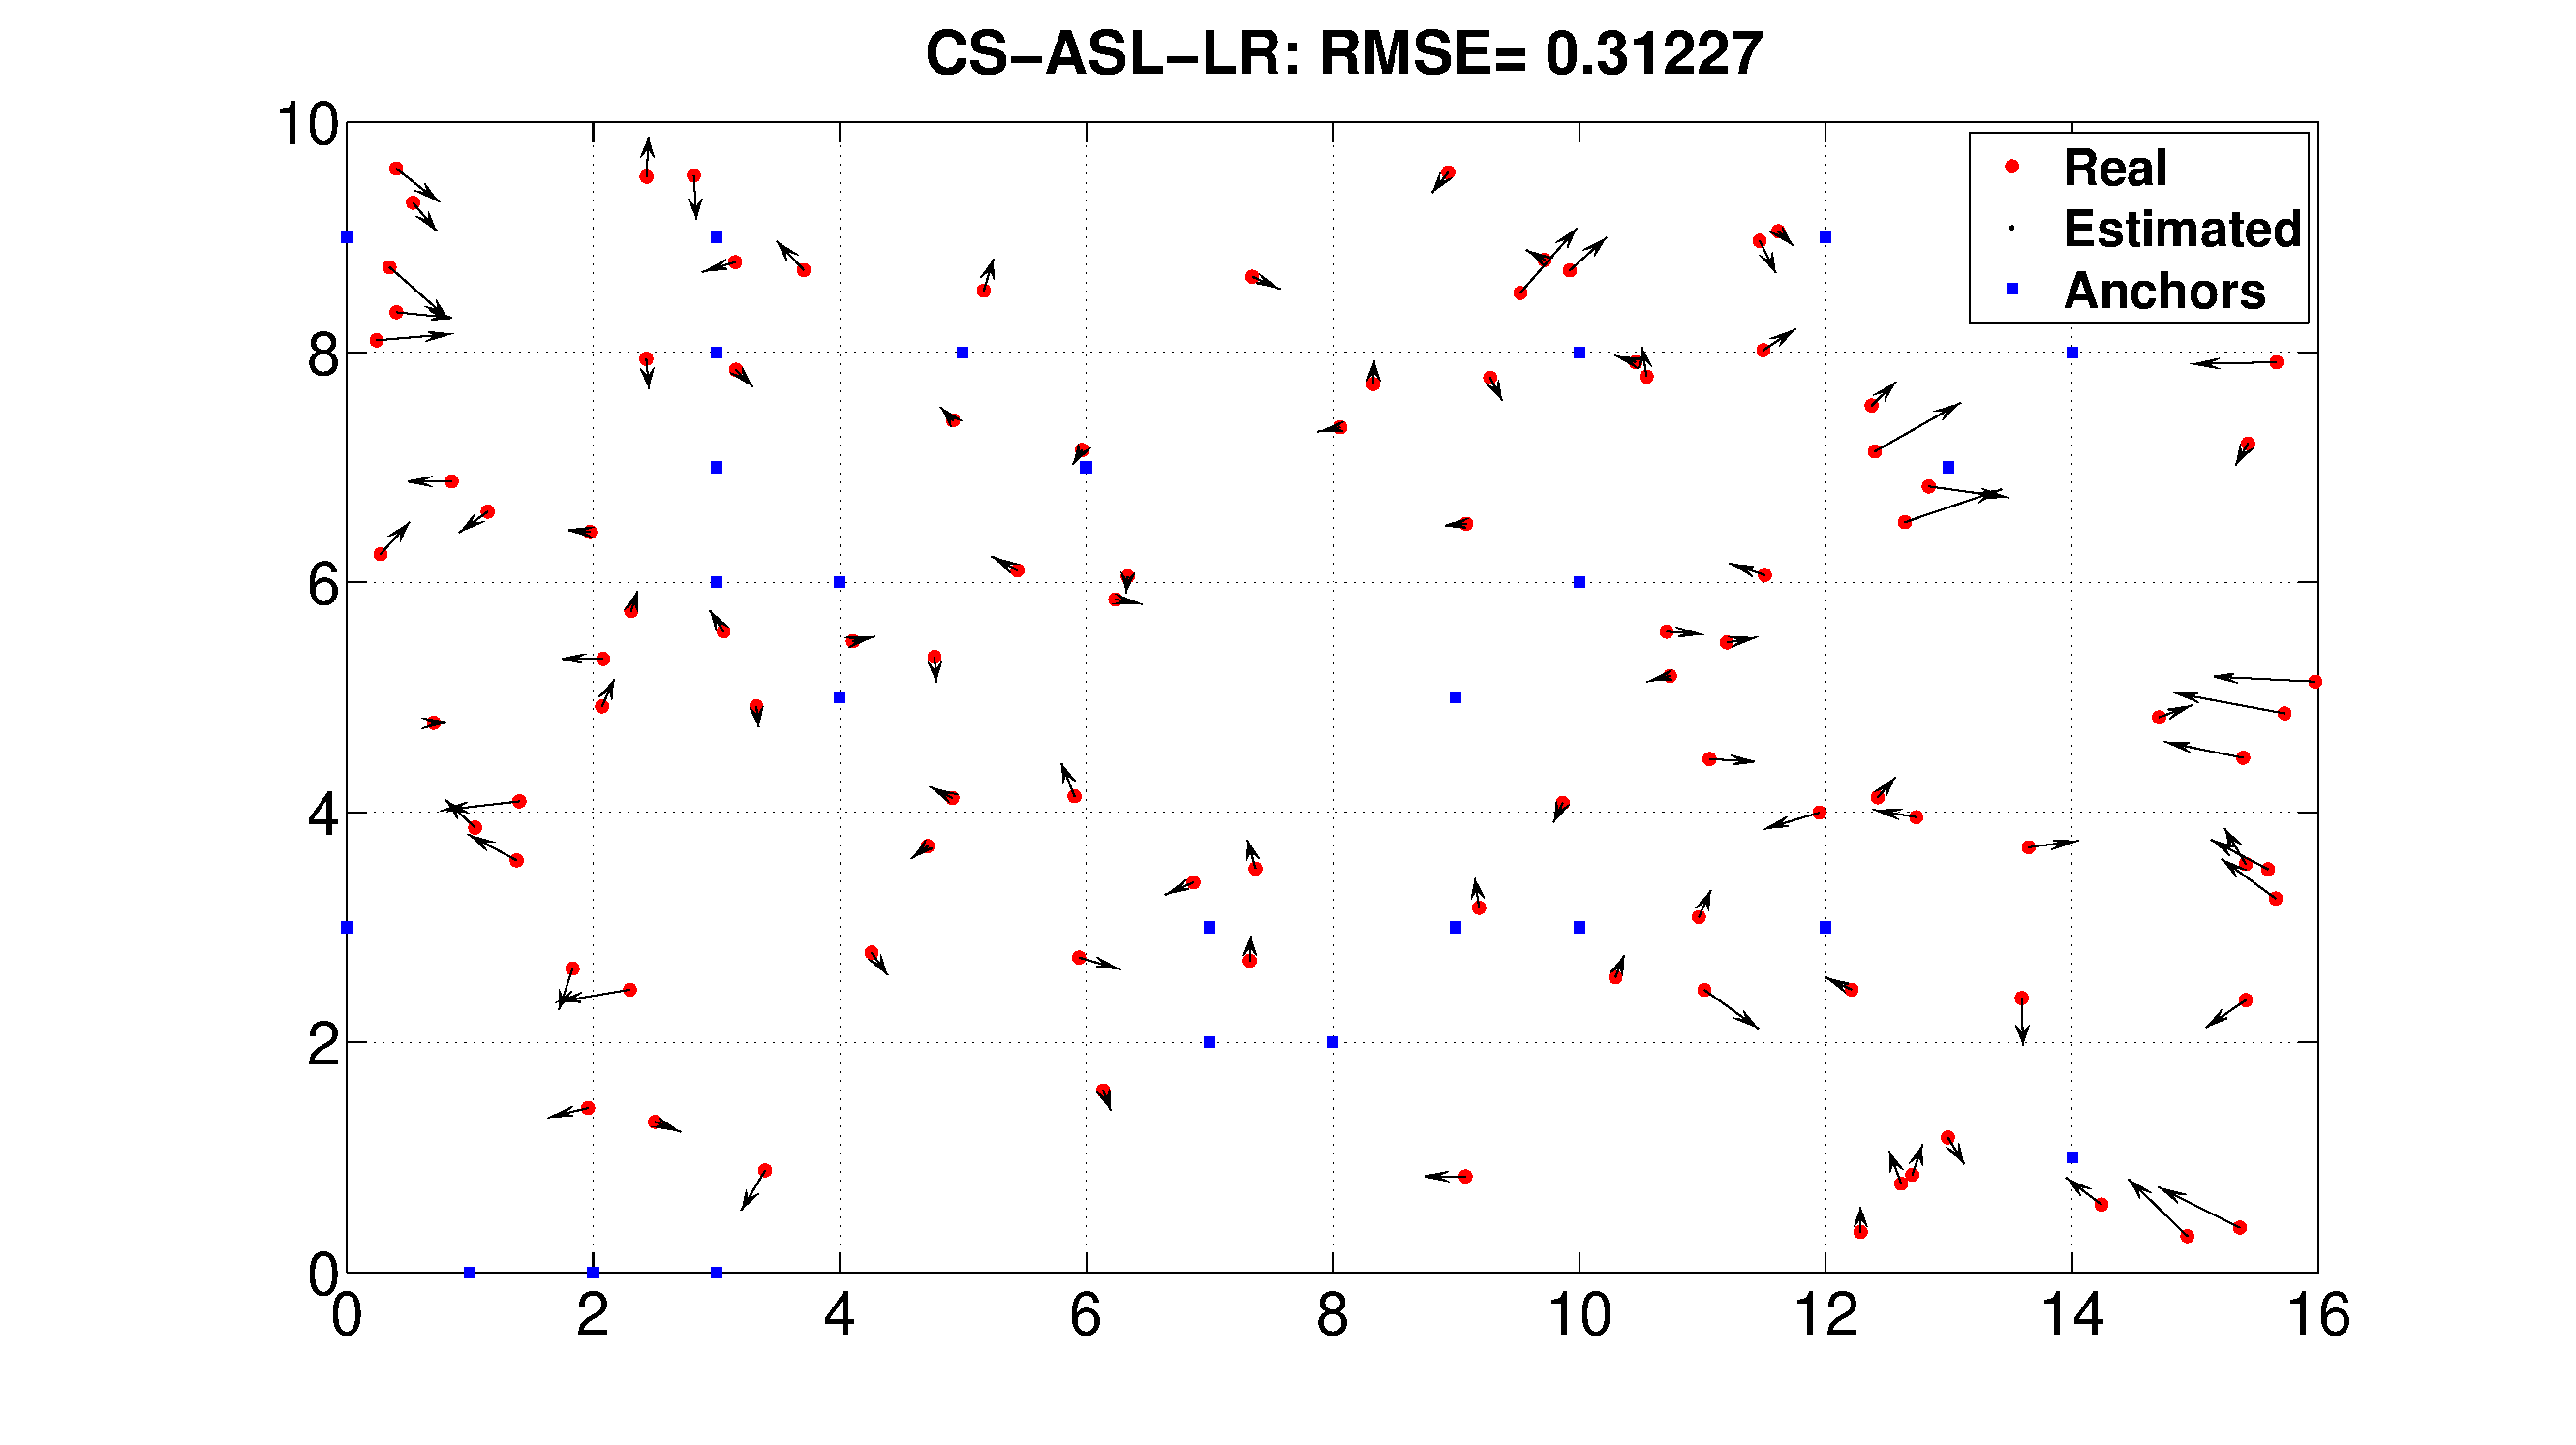
\includegraphics[height=4.5cm]{image/lab.eps} 
	\caption{Testbed experiment}
	\label{overview}
\end{figure} 

 \textbf{Summary:} Considering the parameters including the number of anchors, node location error, angle error and bit-flipping number, simulation results and testbed experiment prove that our methods have a great performance. CS-ASL-BF obtain an accuracy localization result in all fault environment, however, it searches all points every time which slows down the efficiency. CS-ASL-GD based on gradient descent, we make further searching that decrease the final localization error and guarantee the system efficiency even with bit-flipping. CS-ASL-LR takes more step to improve the localization accuracy. Above all, our methods can accomplish localization with robustness.
%%%%%%%%%%%%%%%%%%%%%%%%%%%%%%%%%%%%%%%%%%%%%%%%%

